\documentclass{sagej}

% Load basic packages
\usepackage{balance}		% to better equalize the last page
\usepackage{graphics}		% for EPS, load graphicx instead
\usepackage{times}			% comment if you want LaTeX's default font
\usepackage{url}			% llt: nicely formatted URLs
\usepackage{dblfloatfix}	% allow placement of a page-width figure at top or bottom of page

% llt: Define a global style for URLs, rather that the default one
\makeatletter
\def\url@leostyle{%
  \@ifundefined{selectfont}{\def\UrlFont{\sf}}{\def\UrlFont{\small\bf\ttfamily}}}
\makeatother
\urlstyle{leo}

\usepackage{tikz}
% Make sure hyperref comes last of your loaded packages,
% to give it a fighting chance of not being over-written,
% since its job is to redefine many LaTeX commands.
\usepackage[pdftex]{hyperref}

\newcommand{\modelfraction}{0.65}
\newcommand{\betweenmodels}{0.8cm}

% End of preamble. Here comes the document.
\begin{document}

\title{Performance analysis of a PDEVS simulator supporting multiple synchronization protocols}

\author{Ben Cardoen\affilnum{1}, Stijn Manhaeve\affilnum{1}, Yentl Van Tendeloo\affilnum{1}, and Jan Broeckhove\affilnum{1}}

\affiliation{\affilnum{1}University of Antwerp, Belgium}

\corrauth{Yentl Van Tendeloo
University of Antwerp
Middelheimlaan 1
2020 Antwerp
Belgium}

\email{Yentl.VanTendeloo@uantwerpen.be}

\begin{abstract}
With the ever increasing complexity of simulation models, parallel simulation becomes necessary to perform simulation within reasonable time bounds.
The built-in parallelism of Parallel DEVS is often insufficient to tackle this problem on its own.
Several synchronization protocols have been proposed, each with their distinct advantages and disadvantages.
Due to the significantly different implementation of these protocols, most Parallel DEVS simulation tools are limited to only one such protocol.
In this paper, we present a Parallel DEVS simulator, grafted on C++11 and based on PythonPDEVS, supporting both conservative and optimistic synchronization protocols.
The simulator not only supports both protocols but also has the capability to switch between them at runtime.
We evaluate the performance gain obtained by choosing the most appropriate synchronization protocol.
A comparison is made to adevs in terms of CPU time and memory usage, to show that our modularity does not hinder performance.
We further allow for an external component to gather simulation statistics, on which runtime switching between the different synchronization protocols can be based.
Model allocation is also studied to see how our conservative and optimistic synchronization protocols are affected by good and bad allocations.

\end{abstract}

\maketitle

\section{Introduction}
\label{sec:1-introduction}
\textsf{DEVS}~\cite{ClassicDEVS} is a popular formalism for modelling complex dynamic systems using a discrete-event abstraction.
In fact, it can serve as a simulation ``assembly language'' to which models in other formalisms can be mapped~\cite{DEVSbase}.
A number of tools have been constructed by academia and industry that allow the modelling and simulation of \textsf{DEVS} models.

But with the ever increasing complexity of simulation models, parallel simulation becomes necessary to perform the simulation within reasonable time bounds.
And while \textsf{Parallel DEVS}~\cite{ParallelDEVS} was introduced to increase parallelism, this is often insufficient.
Several synchronization protocols from the discrete event simulation community~\cite{FujimotoBook} have been applied to \textsf{DEVS} simulation.
While several parallel \textsf{DEVS} simulation kernels exist, they are often limited to a single synchronization protocol.
The reason for different synchronization protocols, however, is that their distinct nature makes them applicable in different situations, each outperforming the other in specific models.
The applicability of parallel simulation capabilities of current tools is therefore limited.

This paper introduces DEVS-Ex-Machina\footnote{\url{https://bitbucket.org/bcardoen/devs-ex-machina}} (``dxex''), our simulation tool which offers multiple synchronization protocols: no synchronization (sequential execution), conservative synchronization, or optimistic synchronization.
The selected synchronization protocol is transparent to the simulated model: users should merely determine, which protocol they wish to use.
Users who simulate a wide variety of models, with different ideal synchronization protocols, can simply run the same model with different synchronization protocols.
We investigate in this paper how model allocation and uncertainty determine the choice between synchronization protocols. 
The synchronization overhead is demonstrated by reducing the computational load of a model to near zero. 

Our tool is based on PythonPDEVS, but implemented in C++11 for increased performance, using features from the new C++14 standard when possible.
Unlike PythonPDEVS dxex only supports multicore parallelism.

We implemented a model that, depending on a single parameter, changes its ideal synchronization protocol. We demonstrate using several models the factors influencing the performance under a given synhronization protocol.
Dxex, then, is used to compare simulation using exactly the same tool, but with a varying synchronization protocol. With dxex users can always opt to use the fastest protocol available.
To verify that our flexibility does not counter performance, we compare to adevs, currently one of the fastest \textsf{DEVS} simulation tools available~\cite{PythonPDEVS,DEVSSurvey}.

% Switching and statistics
Dxex offers visualization of the simulation and in depth statistics. A modeller can then make a more informed decision on which synchronization protocol to use or even intervene during simulation and request a switch between protocols. 

%Usage of Hyperref with hardcoded label is hardly ideal, but ~\ref doesn't work if the layout disables numbered sections, so a hack is needed. The alternative is \nameref but that isn't all that readable.
The remainder of this paper is organized as follows:
Section~\hyperref[sec:2-background]{2} introduces the necessary background on synchronization protocols.
Section~\hyperref[sec:3-features]{3} elaborates on our design that enables this flexibility.
In Section~\hyperref[sec:4-performance]{4}, we evaluate performance of our tool by comparing its different synchronization protocols, and by comparing to adevs.
Related work is discussed in Section~\hyperref[sec:5-related-work]{5}.
Section~\hyperref[sec:6-conclusion]{6} concludes the paper and gives future work.


\section{Background}
\label{sec:2-background}
This section briefly introduces the two synchronization protocols used by dxex: conservative and optimistic synchronization.

\subsection{Conservative Synchronization}
The first synchronization protocol we introduce is \textit{conservative synchronization}~\cite{FujimotoBook}.
In conservative synchronization, a node progresses independent of all other nodes, up to the point in time where it can guarantee that no causality errors happen.
When simulation reaches this point, the node blocks until it can guarantee a new time until which no causality errors happen.
In practice, this means that all nodes are aware of the current simulation time of all other nodes, and the time it takes an event to propagate (called \textit{lookahead}).
Deadlocks can occur due to a dependency cycle of models.
Multiple algorithms are defined in the literature to handle both the core protocol, as well as resolution schemes to handle or avoid the deadlocks~\cite{FujimotoBook}.

The main advantage of conservative synchronization is its low overhead if the lookahead is high.
Each node then simulates in parallel, and sporadically notifies other nodes about its local simulation time.
The disadvantage, however, is that the amount of parallelism is explicitly limited by the lookahead.
If a node can influence another (almost) instantaneously, no matter how rarely it occurs, the amount of parallelism is severely reduced.
The user is required to define the lookahead, using knowledge about the model's behaviour.
Defining lookahead is not always a trivial task if there is no detailed knowledge of the model.
Even slight changes in the model can change to the lookahead, and can therefore have a significant influence on simulation performance.

\subsection{Optimistic Synchronization}
A completely different synchronization protocol is \textit{optimistic synchronization}~\cite{TimeWarp}.
Whereas conservative synchronization would prevent causality errors at all costs, optimistic synchronization will allow them to happen, but correct them afterwards.
Each node is allowed to progress in simulated time as much as possible, without taking note of the state of any other node.
When an event arrives at a node, which is already further in simulated time, the node will have to roll back its state to right before the event would normally have to be processed.
As the simulation time is now rolled back to before the event is processed, the event can simply be processed as if no causality error ever occured.

Rolling back the simulation time requires the node to store past model states, such that they can be restored later on.
Furthermore, all incoming and outgoing events need to be stored as well.
Incoming events need to be passed to the models again, when the correct simulation time has again been reached, and outgoing events need to be cancelled, as potentially a different series of output events would normally have been generated.
Cancelling events, however, can cause further rollbacks, as the receiving node might also have to roll back its state.
In practice, a single causality error could have significant repercussions on the complete simulation.

Further changes are required for unrecoverable operations, such as I/O (\textit{e.g.}, tracing, writing to file, printing output) and memory management.
Lightweight algorithms are still required to determine the lower bound of all simulation times, through the computation of a \textit{Global Virtual Time} (GVT).

The main advantage is that performance is not limited by a small lookahead, caused by a very infrequent event.
If an (almost) instantaneous event occurs rarely, performance will only be impacted if it occurs, and not at every simulation step.
The main disadvantage is unpredictable performance and arbitrary cost of rollbacks due to the propagation of causality errors.
If rollbacks occur frequently, simulation quickly becomes slow, as the overhead of the recovery mechanisms becomes significant.
Apart from overhead in CPU time, a significant memory overhead is present: all intermediate states qre stored up to a point where it can be considered \textit{irreversible}.

While optimistic synchronization does not explicitly depends on the lookahead, simulation performance is still bound by the lookahead implicitly.


\section{DEVS-Ex-Machine}
\label{sec:3-features}
Historically, dxex is based on PythonPDEVS~\cite{PythonPDEVS}.
Python is a good language for prototypes, but performance has proven insufficient to compete with other simulation kernels~\cite{MasterThesis}.
Dxex is a C++11-based implementation of PythonPDEVS, but implements only a subset of PythonPDEVS, while making some of its own additions.
So while the feature set is not too comparable, the architectural design, core simulation algorithm, and optimizations, are highly similar.

We will not make a detailed comparison with PythonPDEVS here, but only mention some supported features.
Dxex supports, similarly to PythonPDEVS, the following features: direct connection~\cite{SymbolicFlattening}, \textsf{Dynamic Structure DEVS}~\cite{DSDEVS}, termination conditions, and a modular tracing and scheduling framework~\cite{PythonPDEVS}.
But whereas PythonPDEVS only supports optimistic synchronization, dxex support multiple synchronization protocols (though only in parallel).
This is in line with the design principle of PythonPDEVS: allow users to pass performance hints to the simulation kernel.
In our case, a user can pass the simulation kernel sets the synchronization protocol to be used for this model.
Our implementation in C++11 also allows for optimizations which were plainly impossible in an interpreted language.

Since there is no universal \textsf{DEVS} model standard, dxex models are incompatible with PythonPDEVS and vice versa.
This is due to dxex models being grafted on C++11, whereas PythonPDEVS models are grafted on Python.

In the remainder of this section, we will elaborate on our prominent new feature: support for multiple synchronization protocols within the same simulation tool, which are offered transparently to the model.

\subsection{Synchronization protocols}
We previously explained the existence of different synchronization protocols exist, each optimized for a specific kind of model.
As no single synchronization protocol is ideal for all models, a general purpose simulation tool should support multiple protocols.
Currently, most parallel simulation tools choose only a single synchronization protocol due to the inherent differences between protocols.
An uninformed choice on which one to implement is insufficient, as performance will likely be bad.
We argue that a real general purpose simulation tool should support sequential, conservative, and optimistic synchronization, as is the case for dxex.

These different protocols relate to three different model characteristics.
Conservative synchronization for when high lookahead exists between different nodes, and barely any blocking is necessary.
Optimistic synchronization for when lookahead is unpredictable, or there are rare (almost) instantaneous events.
Finally, sequential simulation is still required for models where parallelism is bad, where all protocols actually slow down simulation.

\subsubsection{Sequential}
Our sequential simulation algorithm is very similar to the one found in PythonPDEVS, including many optimizations.
Minor modifications were made, though, such that it can be overloaded by different synchronization protocol implementations.
This way, the \textsf{DEVS} simulation algorithm is implemented once, but parts can be overridden as needed.
In theory, more synchronization protocols (\textit{e.g.}, other algorithms for conservative synchronization) can be added without altering our design.

An overview of dxex's design is given in Figure~\ref{fig:class_diagram}.
It shows that there is a simulation \texttt{Core}, which simulates the \texttt{AtomicModel}s connected to it.
The superclass \texttt{Core} is merely the sequential simulation core, but can be used as-is.
Subclasses define specific variants, such as \texttt{ConservativeCore} (conservative synchronization), \texttt{OptimisticCore} (optimistic synchronization), and \texttt{DynamicCore} (\textsf{Dynamic Structure DEVS}).

\begin{figure}
    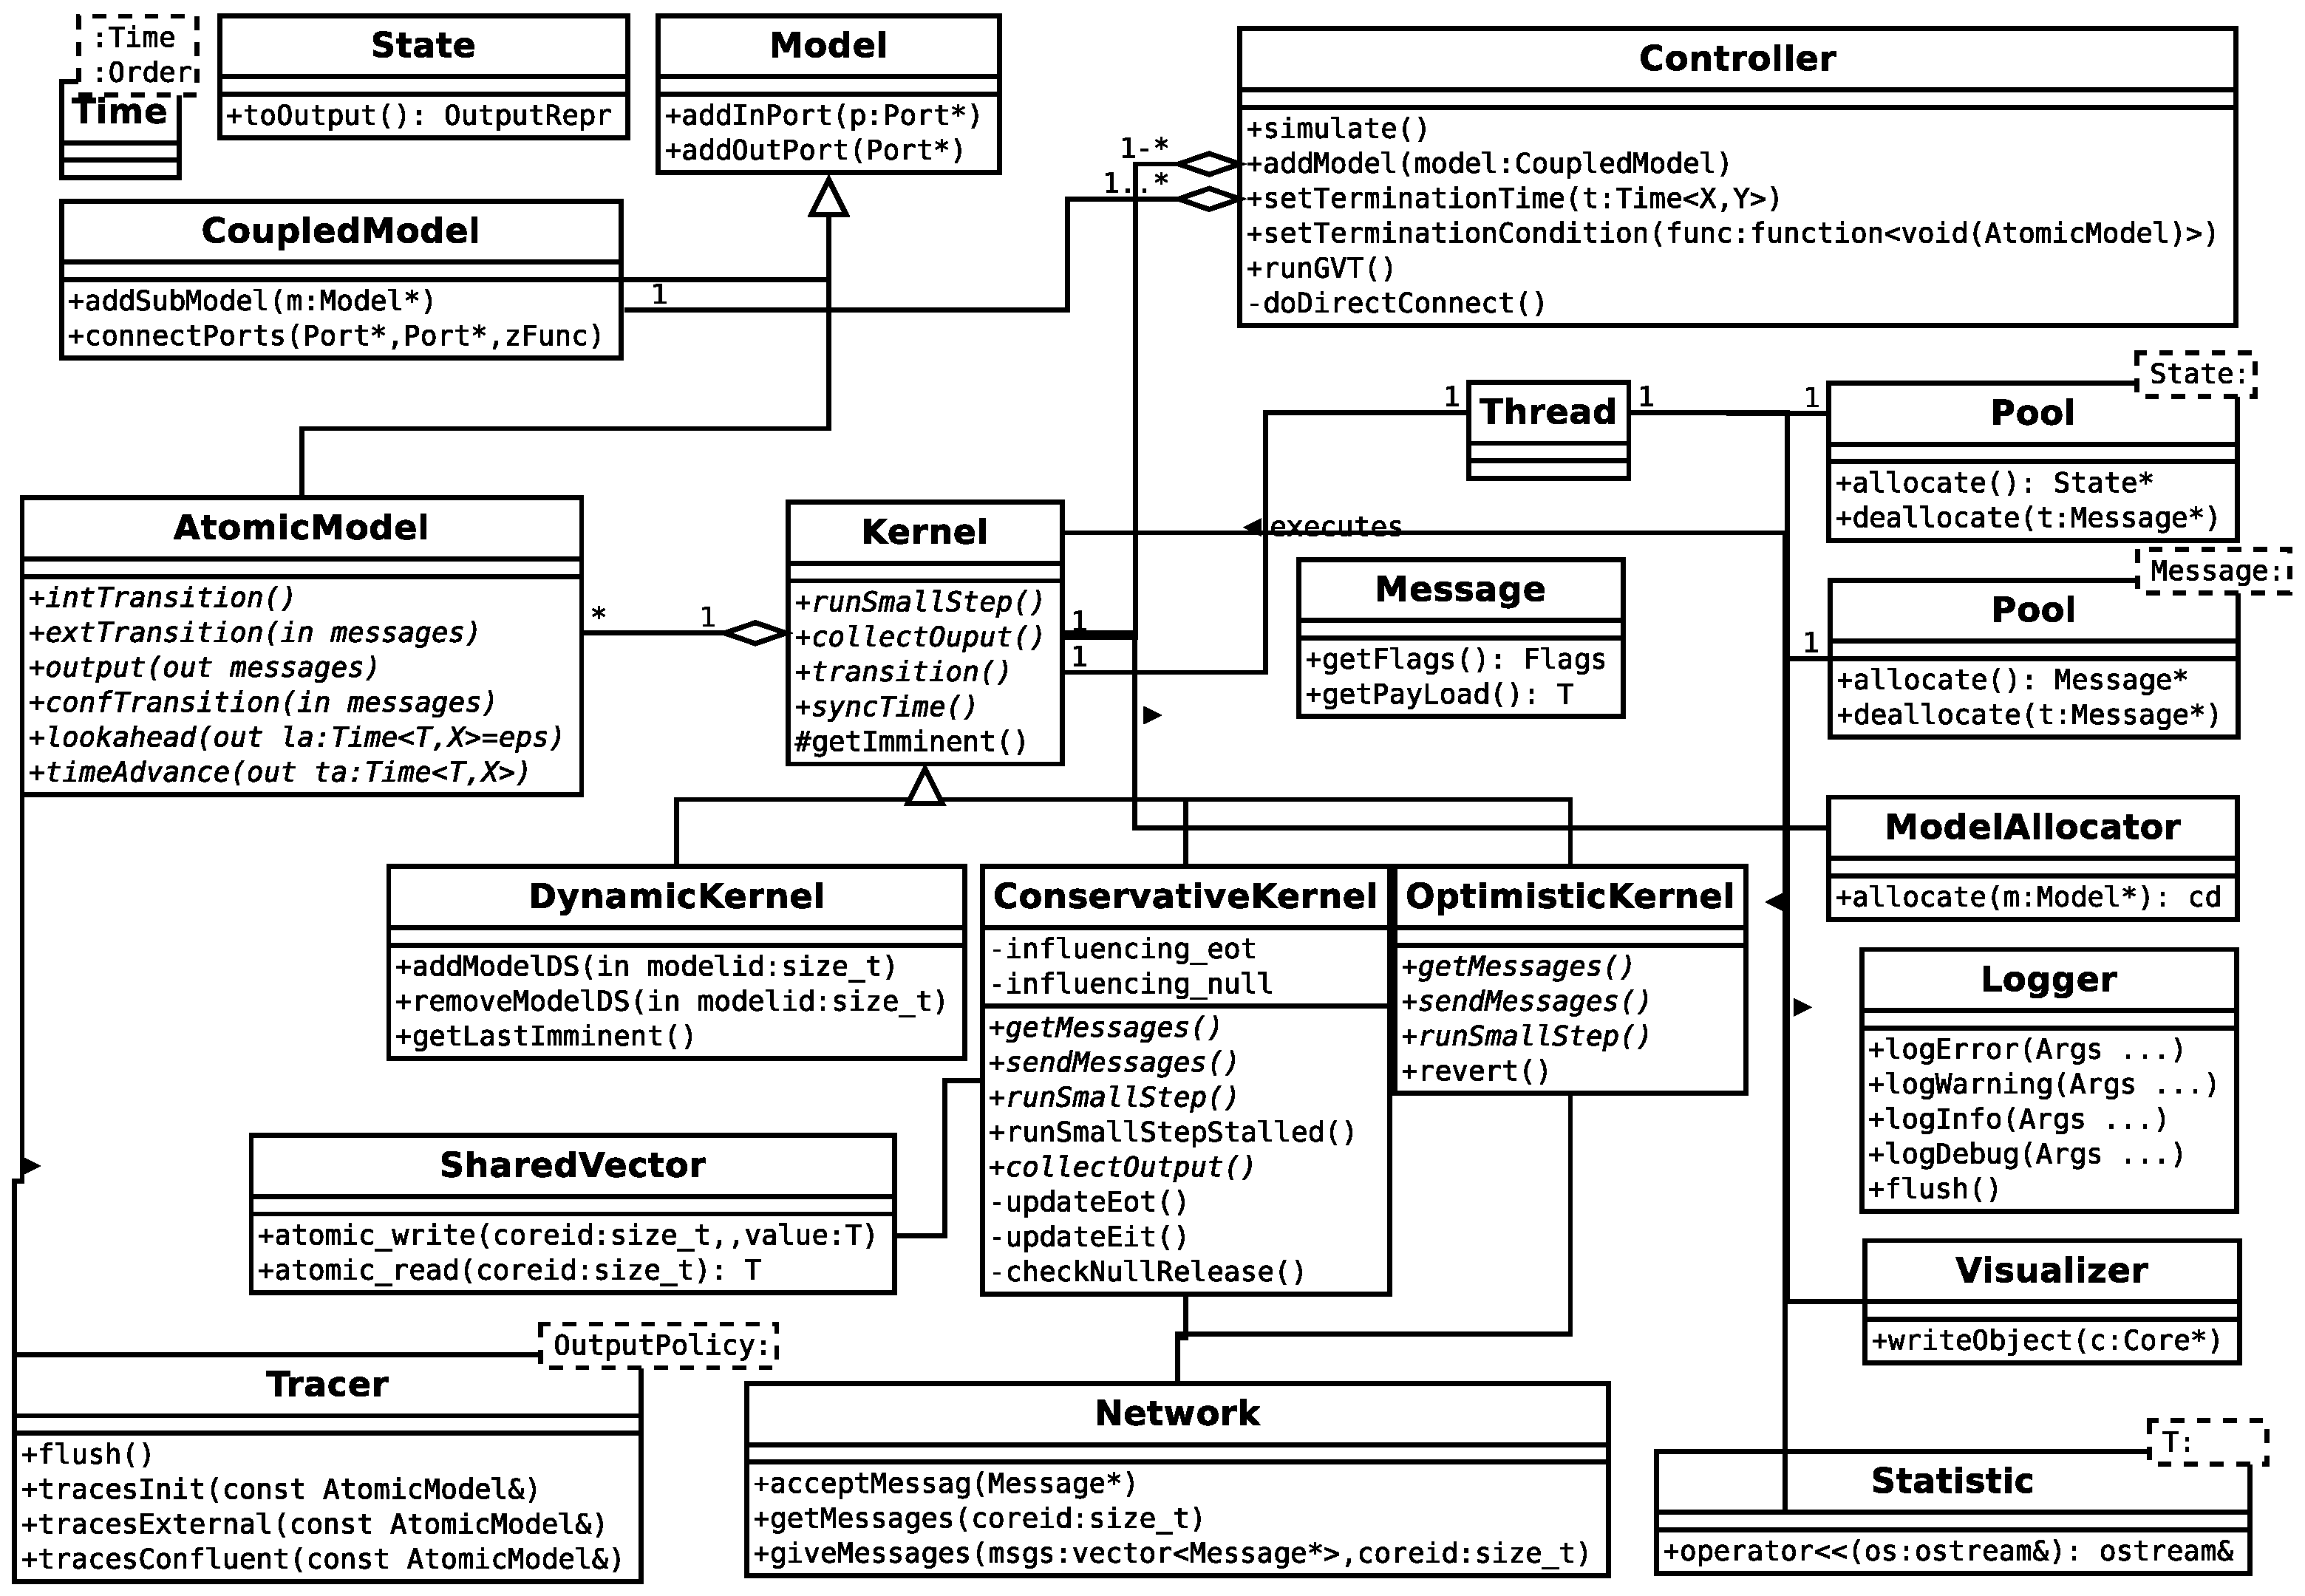
\includegraphics[width=\columnwidth]{fig/cores_class_diagram.eps}
	\caption{Dxex kernel design.}
	\label{fig:class_diagram}
\end{figure}

\subsubsection{Conservative}
For conservative synchronization, each node must determine the nodes it is influenced by.
Each model needs to provide a lookahead function, which determines the lookahead depending on the current simulation state.
Within the returned time interval, the model promises not to raise an event.
A node aggregates this information to computes its earliest output time (EOT).
This value is written out in shared memory, where it can be read out by all other nodes.

Reading and writing to shared memory is done through the use of the new C++11 synchronization primitives.
Whereas this was also possible in previous versions of the C++ standard, by falling back to non-portable C functions, it was not a part of the C++ language standard.
C++11 further allows us to make the implementation portable, as well as more efficient: the compiler might know of optimizations specific to atomic variables.

\subsubsection{Optimistic}
For optimistic synchronization, each node must be able to roll back to a previous point in time.
This is often implemented through the use of state saving.
This needs to be done carefully in order to avoid unnecessary copies, and minimize the overhead.
We use the default: explicitly save each and every intermediate state.
Mattern's algorithm~\cite{mattern} is used to determine the GVT, as it runs asynchronously and uses only $2n$ synchronization messages.
Once the GVT is found, all nodes are informed of the new value, after which fossil collection is performed, and irreversible actions are committed.

The main problem we encountered in our implementation is the aggressive use of memory.
Frequent memory allocation and deallocation caused significant overheads, certainly when multiple threads do so concurrently.
This made us switch to the use of thread-local (using \texttt{tcmalloc}) memory pools.
Again, we made use of specific new features of C++11, that were not available in Python, or even previous versions of the C++ language standard.

\subsection{Transparency}
We define simulation kernel transparency as having a single model, which always can be executed on each supported synchronization kernel, without any modifications.
User should thus only provide one model, implemented in C++11, which can be either using sequential execution, using conservative synchronization, or using optimistic synchronization.
Switching between simulation kernels is as simple as altering the simulation termination time.
The exception is conservative synchronization, where a lookahead function is required, which is not used in other synchronization kernels.
Two options are possible: either a lookahead function must always be provided, even when it is not required and possibly not used, or we use a default lookahead function if none is defined.

Always defining a lookahead function might seem redundant, especially if users will never use conservative synchronization.
Especially since defining the lookahead is often non-trivial and dependent on intricate model details.
The more attractive option is for the simulation tool to provide a default lookahead function, such that simulation can run anyway, but maybe not at peak performance.
%Depending on the model, simulation performance might still be faster than sequential simulation. 

Defining a lookahead function is therefore recommended in combination with conservative synchronization, but is not a necessity, as a default of $epsilon$ can be used otherwise.


\section{Performance Evaluation}
\label{sec:4-performance}
% DESIGN OF MODELS
\section{Atomic models}

\section{Coupled models}

% SEQUENTIAL
\subsection{Sequential Simulation}
We start by evaluating sequential simulation performance, in order to obtain a baseline for our comparison of parallel simulation performance.

\subsubsection{Queue}
\label{4-seq-Queue}
% explain what we did: fixed number of models (400, 600 & 800), increasing depth
For the first benchmark, we tested the effect of hierarchical complexity of the model in the performance of the simulator.
A set of three tests was performed, where each test has the same number of models but an increasing depth.
The results can be seen in Figure~\ref{fig:Queue_benchmark_seq}.
Since dxex symbolically flattens the model, there is no performance hit when the depth is increased.
The overhead of running the directconnect algorithm is one time only and negligible when the end time of the simulation is sufficiently large.
Adevs on the other hand does suffer from the increased depth.
With every new hierarchical layer, routing an event from one atomic model to the next becomes more expensive, resulting in an increase in runtime.
\begin{figure}
	\center
	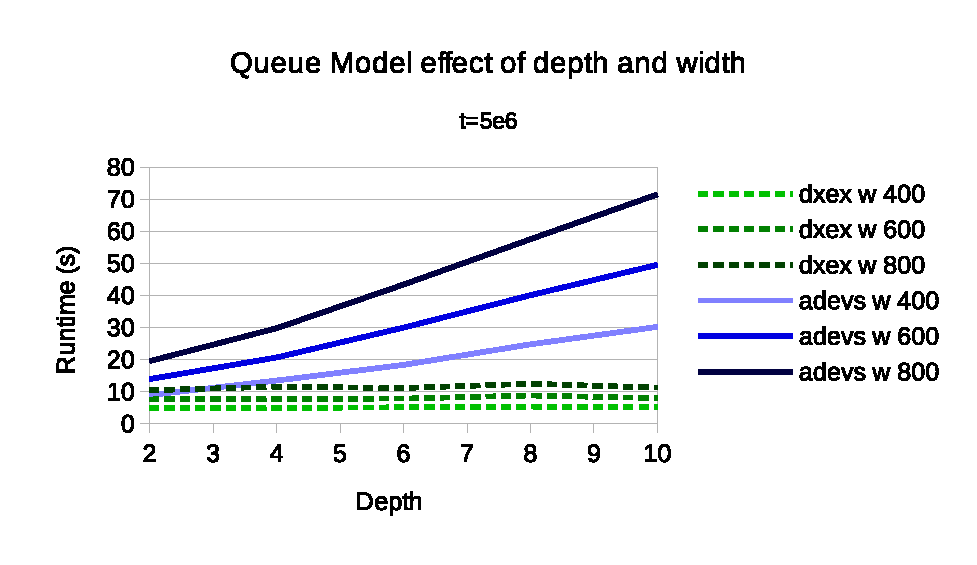
\includegraphics[width=\columnwidth]{fig/queue_fixed_sequential.eps}
	\caption{Queue benchmark results for sequential simulation.}
	\label{fig:Queue_benchmark_seq}
\end{figure}

\subsubsection{Interconnect}
\label{4-seq-Interconnect}
In the Interconnect model, we increase the number of atomic models, thus quadratically increasing the number of couplings and the number of external transitions.
As can be seen in Figure~\ref{fig:Interconnect_benchmark}, adevs outperforms dxex by a fair margin.
Analysis showed that this is caused by the high amount of events: event creation is much slower in dxex than it is in adevs, despite dxex's use of memory pools.
To shield the user from threading and deallocation concerns dxex provides an event superclass from which the user can derive to create a specialized event type.
Copying and deallocation semantics and tracing are solved by the kernels at a runtime cost in simulations where event frequency is very high.
Profiling the benchmarks clearly shows the increasing cost of output generation and deallocation as the determining factor in the gap in performance.
We refer the interested reader to the dxex \hyperref{https://bitbucket.org/bcardoen/devs-ex-machina}{}{repo}{repository} for the profiling call graphs for the different benchmarks.

\begin{figure}
	\center
	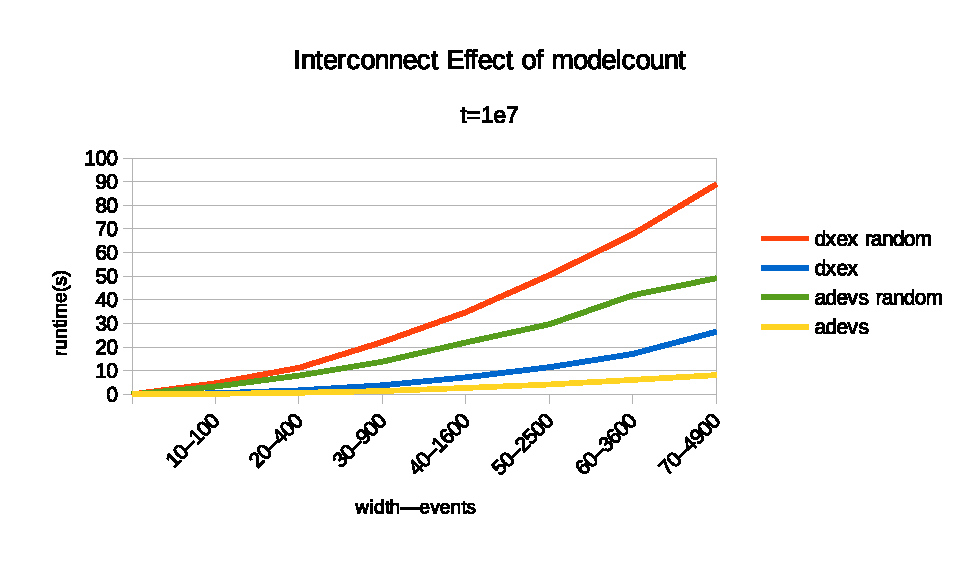
\includegraphics[width=\columnwidth]{fig/interconnect_sequential.eps}
	\caption{Interconnect benchmark results for sequential simulation.}
	\label{fig:Interconnect_benchmark}
\end{figure}

\subsubsection{PHold}
\label{4-seq-PHold}
The PHold model is very similar to the Interconnect model.
The biggest difference is that the amount of messages sent is much lower.
The number of events scales linear with the number of models, not quadratic.
Figure~\ref{fig:Phold_benchmark} shows that the performance of dxex and adevs are very close to each-other, with adevs slightly outperforming dxex.
\begin{figure}
	\center
	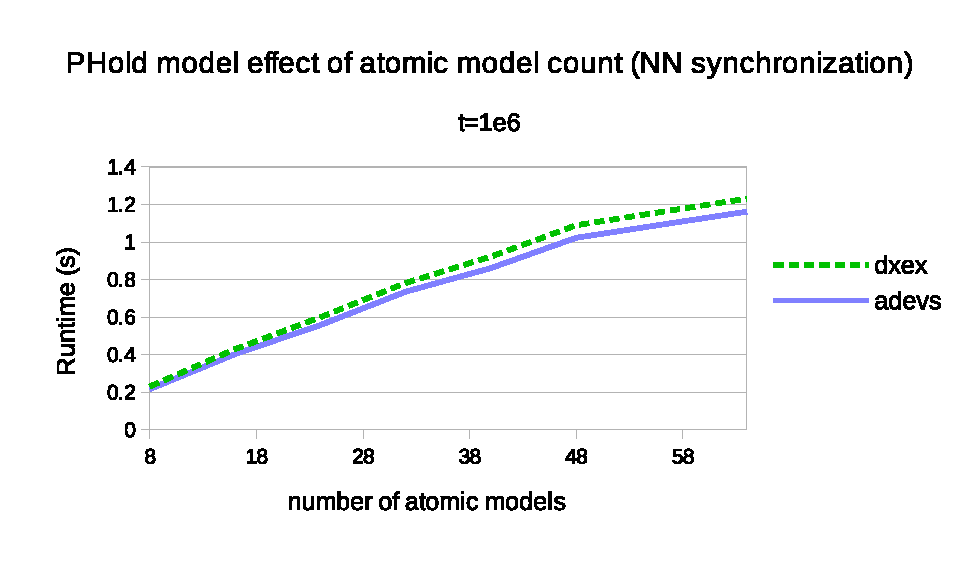
\includegraphics[width=\columnwidth]{fig/phold_sequential.eps}
	\caption{PHold benchmark results for sequential simulation.}
	\label{fig:Phold_benchmark}
\end{figure}


% PARALLEL
\subsection{Parallel Simulation}

% The good
\subsubsection{Queue}
\paragraph*{Allocation}
The Queue model is one single chain of models. Each kernel gets one connected part of this chain. The result is that the kernels themselves also form a chain where events only travel in one direction.

\paragraph*{Strong and Weak Scaling}
Figure~\ref{fig:Queue_plot_strong} shows the speedup compared to dxex sequential for a fixed problem size. As the amount of kernels increases, the optimistic kernel quickly becomes the worst choice. The difference between dxex conservative and adevs becoming smaller. The same effect can be seen for weak scaling in Figure~\ref{fig:Queue_plot_weak}.\\
In Figure \ref{fig:Queue_allocation} the allocation of the Queue model is visualized. This trace allows us to demonstrate the benchmark results and explain why optimistic is not ideal for such a chain topology as present in Queue. Kernel 2 is dependent on events from kernels 0 and 1 but by definition of the optimistic synchronization protocol it will simulate ahead without waiting for events it depends on. Any simulation it performs will have to be reverted as soon as events from kernels 0 and 1 arrive. When kernel 2 reverts, kernel 3 will inevitably have to revert as well since most of the events it received from kernel 2 are invalidated and marked as such by antimessages. This leads to severe performance degradation, with an increasing probability of cascading reverts as the number of kernels and models per kernels increases.
The speedup of adevs is always in comparison with the runtime of the corresponding dxex sequential benchmark.
\begin{figure}
	\center
	
	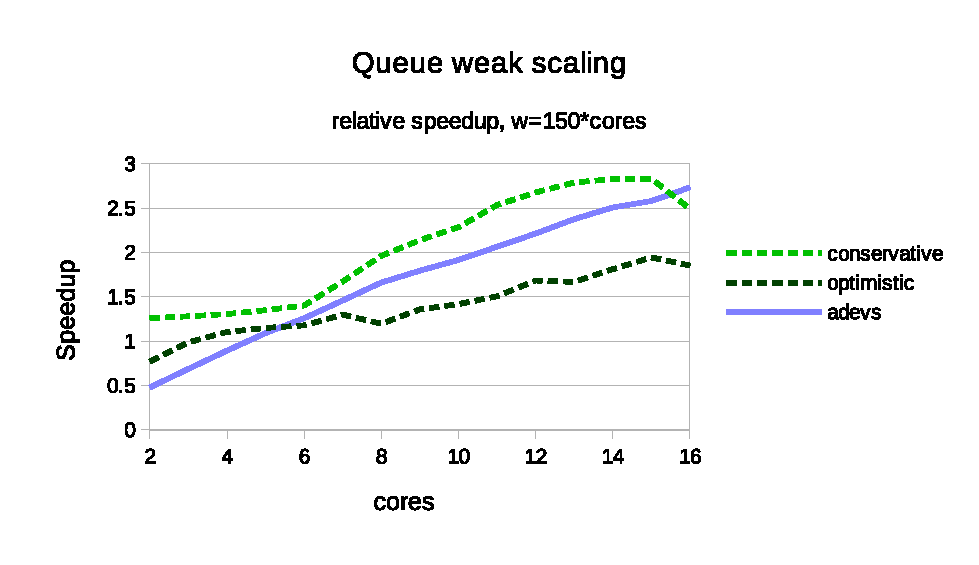
\includegraphics[width=\modelfraction\columnwidth]{fig/queue_fixed_weak_speedup.eps}
	\caption{Queue model weak scaling speedup compared to dxex sequential.}
	\label{fig:Queue_plot_weak}
	
	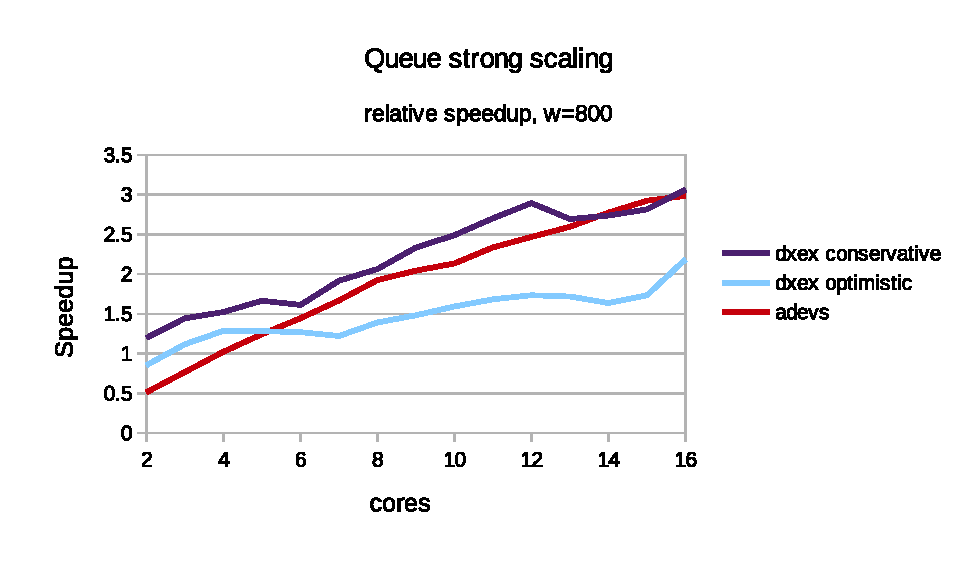
\includegraphics[width=\modelfraction\columnwidth]{fig/queue_fixed_strong_speedup.eps}
	\caption{Queue model strong scaling speedup compared to dxex sequential.}
	\label{fig:Queue_plot_strong}
		
\end{figure}

\begin{figure}
	\center
	
	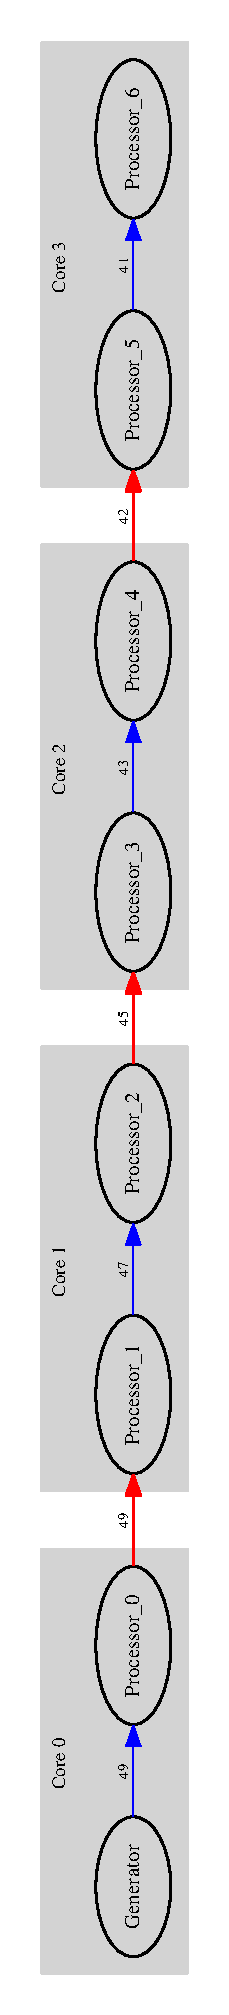
\includegraphics[width=\modelfraction\columnwidth, height=8cm, keepaspectratio, angle=-90 ]{fig/queue_allocation.eps}
	\caption{Queue model (d=2, w=7, t=5000, random timeadvance) allocation and simulation trace across 4 kernels.}
	\label{fig:Queue_allocation}
	
\end{figure}

% The really bad
\subsubsection{Interconnect}\label{subsec:parallelinterconnect}
In the Interconnect model, we determine how broadcast communication is supported across multiple nodes.
The number of models is now kept constant at eight.
Results are shown in Figure~\ref{fig:interconnect_benchmark_parallel}.
When the number of nodes increases, performance decreases due to increasing contention in conservative simulation and an increasing number of of rollbacks in optimistic simulation.
All models depend on each other and have no computational load whatsoever, negating any possible performance gain by executing the simulation in parallel.
In Interconnect there is no allocation scheme possible that avoids cyclic dependencies between simulation kernels, as shown in the trace \ref{fig:interconnect_allocation_parallel} of a simulation with 4 models. Such a cycle forces sequential operation of the kernels with no speedup possible.

\begin{figure}
	\center
	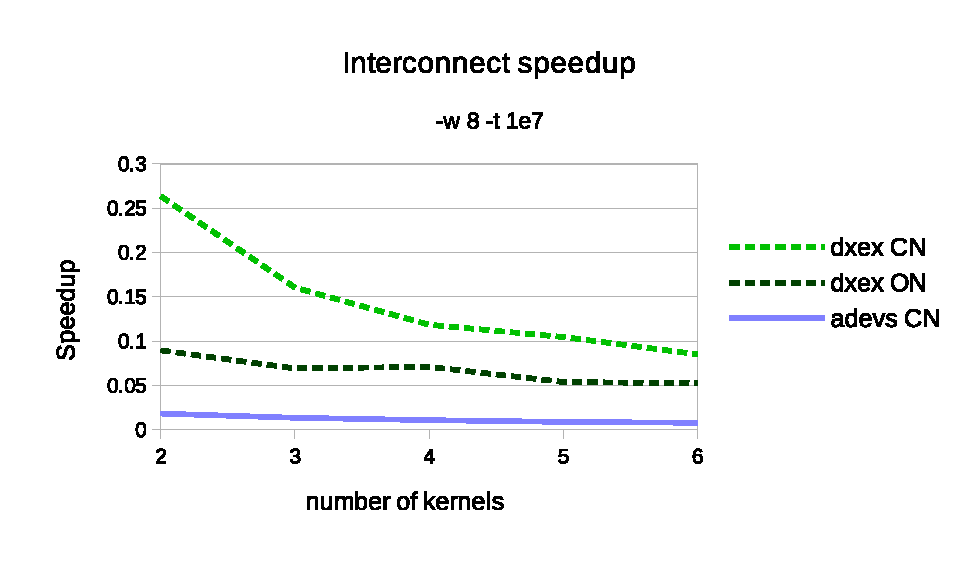
\includegraphics[width=\plotfraction\columnwidth]{fig/interconnect_parallel.eps}
	\caption{Interconnect benchmark results for parallel simulation.}
	\label{fig:interconnect_benchmark_parallel}
\end{figure}
\begin{figure}
	\center
	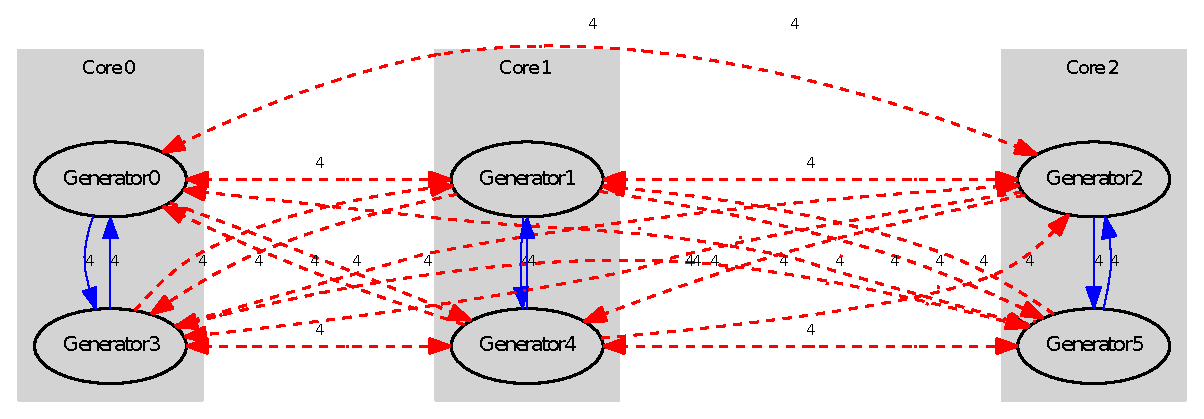
\includegraphics[width=\plotfraction\columnwidth]{fig/interconnect_parallel_allocation.eps}
	\caption{Interconnect parallel simulation trace for 6 models on 3 kernels.}
	\label{fig:interconnect_allocation_parallel}
\end{figure}

% The okayish
\subsubsection{Phold}
% Same cause, different results
In the Phold model, we first investigate the influence of the percentage of remote events on the speedup. A remote event in this context is an event that is sent from a model on one kernel to a model on another simulation kernel.
When remote events are rare, optimistic synchronization rarely has to roll back, thus increasing performance.
With more common remote events, however, optimistic synchronization quickly slows down due to frequent rollbacks.
Conservative synchronization, on the other hand, is mostly unconcerned with the number of remote events: the mere fact that a remote event can happen, causes it to block and wait.
Even though a single synchronization protocol is always ideal in this case, it already shows that different synchronization protocols respond differently to a changing model.
Adevs is significantly slower during conservative synchronization.
Analysis of profiling callgraphs shows that exception handling in adevs is the main cause. 
To keep the models equivalent, the adevs version does not provide the \{begin,end\}Lookahead methods, which accounts for the exception handling. These functions require the user to implement a state saving in contrast to PythonPDEVS and dxex's optimistic kernels which handle this inside the kernel. We feel this would lead to an unfair comparison as we would like to keep the models synchronization-agnostic across all benchmarks.

\begin{figure}
    \center
    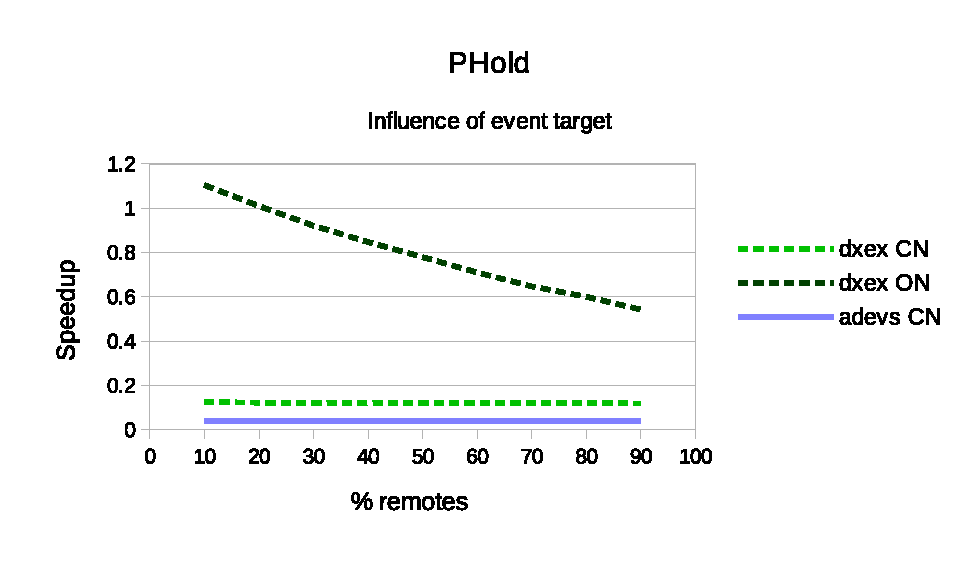
\includegraphics[width=\plotfraction\columnwidth]{fig/phold_remotes.eps}
    \caption{Phold benchmark results for parallel simulation using four kernels, four atomics per node, with varying percentage of remote events.}
\end{figure}
\begin{figure}
	\center
	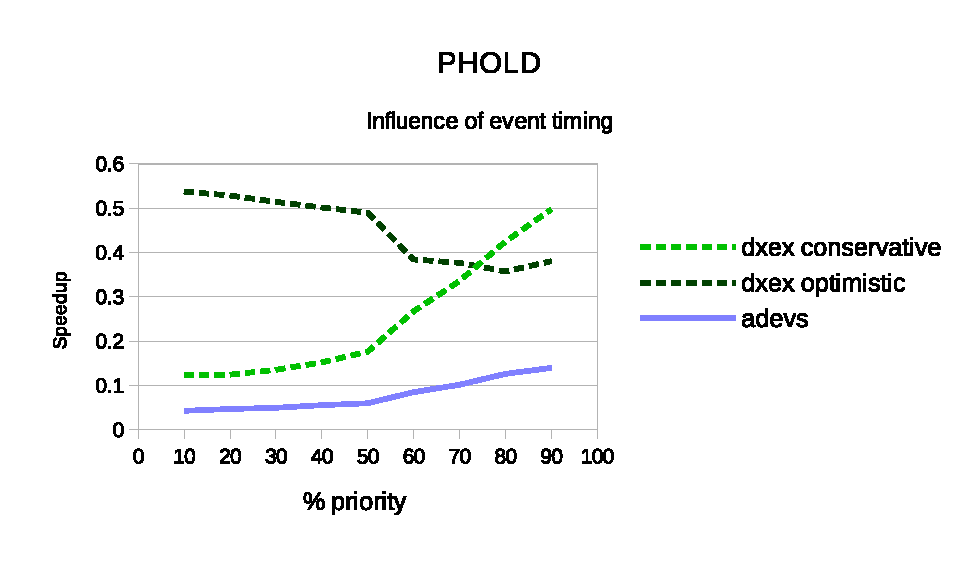
\includegraphics[width=\plotfraction\columnwidth]{fig/phold_priority.eps}
	\caption{Phold benchmark results for parallel simulation using four kernels, with varying amount of high-priority events.}
	\label{fig:phold_priority}
\end{figure}
\begin{figure}
	\center
	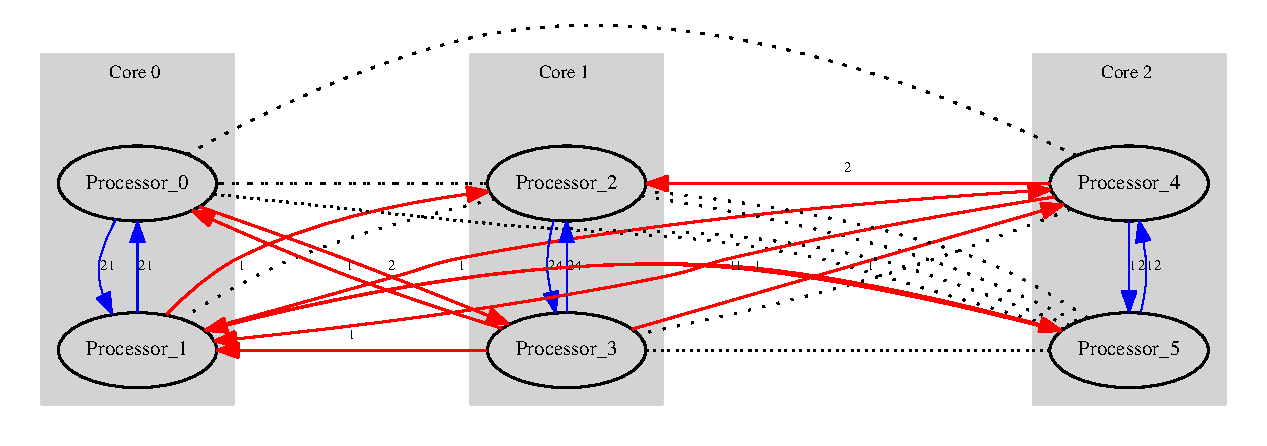
\includegraphics[width=\plotfraction\columnwidth]{fig/phold_parallel_allocation.eps}
	\caption{Phold benchmark trace for parallel simulation using three kernels.}
	\label{fig:phold_allocation}
\end{figure}

We slightly modified the Phold benchmark, to include high-priority events.
Contrary to normal events, high-priority events happen almost instantaneously, restricting lookahead to a very small value.
Even when normal events occur most often, conservative synchronization always blocks until it can make guarantees.
Optimistic synchronization, however, simply goes forward in simulation time and rolls back when these high-priority events happen.
This situation closely mimics the case made in the comparison between both synchronization algorithms by~\cite{FujimotoBook}.
In Figure \ref{fig:phold_allocation} it is clear that in Phold it is possible for dependency cycles to form between kernels which as we have shown in Interconnect degrades performance for both optimistic and conservative. This is also the cause of the sublinear speedup observed in our Phold benchmark.

Figure~\ref{fig:phold_priority} shows how simulation performance is influenced by the fraction of these high-priority events.
If barely any high-priority events occur, conservative synchronization is penalized due to its excessive blocking, which often turned out to be unnecessary.
When many high-priority events occur, optimistic synchronization is penalized due to its mindless progression of simulation, which frequently needs to be rolled back.
Results show that there is no single perfect synchronization algorithm for this model: depending on configuration, either synchronization protocol might be better.


\subsection{Comparison with PDEVS}
In this section we contrast the speedup between the original PDEVS algorithm and the synchronization protocols. 
Note that the PDEVS algorithm and the synchronization protocols are complementary in \textit{dxex}, not exclusive. 
Following the theoretical analysis published in ~\cite{amdahlpdevs} a comparison between PDEVS and the synchronization protocols was warranted. 
We compare the ideal scenario for PDEVS where all events are concurrent with a scenario where events are random.
In this work we do not consider the distribution of events, introducing a random number generator as we will show in this work can mask performance results. 
By limiting ourselves to the best and worst case scenario we demonstrate the capabilities and limitations of both approaches.
The influence of the computational load of the transition functions is a second factor we investigate in this section.
We are interested in scenarios where PDEVS and the synchronization protocols can complement each other in addition to observing their speedup in isolation.
The benchmarks are run on the same hardware as our previous results, a 8 x AMD Opteron(TM) Processor 6274 machine with 8 cores per cpu (64 cores) and 192 GB RAM. 
The benchmarks use a maximum of 16 threads to be divided between PDEVS , conservative or optimistic. 

\paragraph{Model}
As shown in the previous section, when most models are dependent on each other across kernels there is no speedup obtainable by either optimistic or conservative. 
We therefore opted to use the \textit{Queue} model in this benchmark, with depth 4 and width 300.
The effect of combining 4 synchronized kernels with each 4 threads for PDEVS is contrasted with 16 threads for PDEVS and 16 kernels for conservative and optimistic.  
This allows us to observe which is more efficient in obtaining a speedup.
We simulate a computational load by a call to sleep in the transition functions set at 5ms. 

\paragraph{Concurrent events}
First we create the ideal scenario for PDEVS, all events are concurrent with a significant computational load in the transition functions. 

In figure \ref{fig:pdevs_plot_fixed_sleep} we observe that PDEVS obtains a speedup approaching 8. 
Conservative and optimistic are run first with 16 kernels, then with 4 kernels having 4  PDEVS threads each. 
The resulting speedup is half of that obtained of the sequential kernel with 16 PDEVS threads.

\paragraph{Random events}
Random events allow us to demonstrate the overhead of PDEVS. The probability that events are concurrent is strongly reduced.
The transition function has the same computational load as in the previous configuration. 
The results in figure \ref{fig:pdevs_plot_random_sleep} demonstrate that the overhead in the sequential DPEVS kernel is negligible. In contrast both conservative and optimistic suffer a significant slowdown when combined with PDEVS.
We clearly see that conservative and optimistic outperform the sequential kernels in this scenario, complementing the synchronized kernels with PDEVS is not warranted here.

\paragraph{Computational load}
When we remove the computational load we isolate the overhead of the parallelism. 
In this paper we are mainly interested in this overhead which is otherwise masked by adding a computational cost to the transition functions. 
All the benchmarks in this work are run with a near negligible computational load in the transition functions for this purpose.
If a parallel speedup can be obtained in a simulation model without any load in the transition function this will translate in a higher speedup with an increased load, as this load can then be spread over kernels or threads.
Although this configuration has only concurrent events the overhead of the synchronization is severe. 
The runtime cost of this overhead is extreme in the sequential kernel. 
The synchronized kernels are impacted less by the overhead of the PDEVS algorithm.
 
\paragraph{Discussion}
In \textit{dxex} PDEVS and the two synchronization protocols are complementary. The user is not forced to choose between either but can divide the capabilities of his machine over both approaches.
While PDEVS can offer a significant speedup we see that to offer this speedup the concurrency of events must be significant in combination with a high computational load in the transition functions. 
We measure the overhead introduced by PDEVS to give practitioners insight into which model can benefit from which paradigm.
The overhead of the synchronization protocols in specific scenarios  is shown in the previous section.
For a given model it is difficult to predict the concurrency of events, although the computational load of a transition function can be approximated.
In these benchmarks we show which configurations can lead to a speedup for PDEVS or the synchronization protocols in isolation or combination.
In \citep{amdahlpdevs} a theoretical bound is defined for the maximum speedup obtained by PDEVS. 
Our tool flattens the hierarchy of the coupled models


\begin{figure}
	\center
	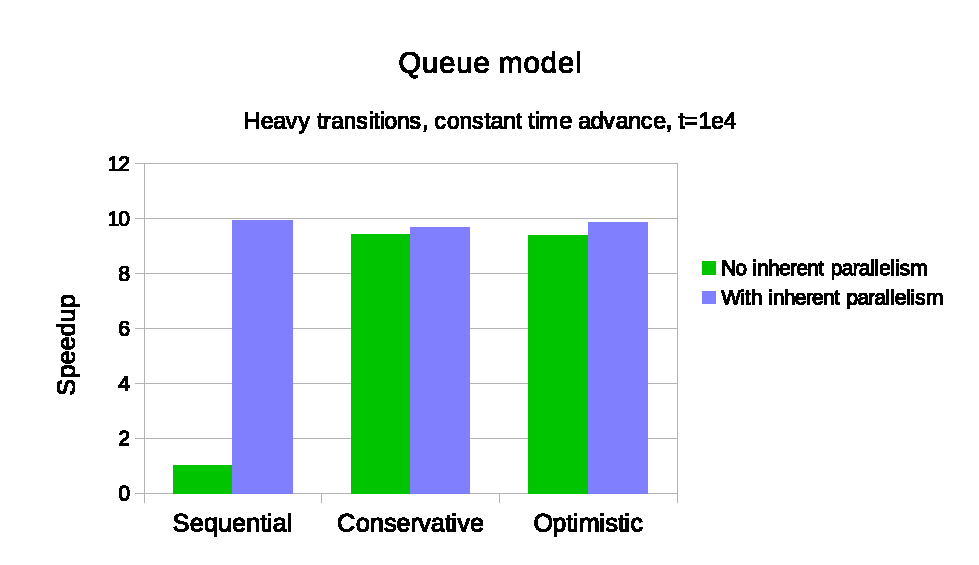
\includegraphics[width=\columnwidth]{fig/pdevs_fixed_sleep.eps}
	\caption{Queue speedup benchmark for PDEVS and synchronization with maximal concurrent events and significant computational load}
	\label{fig:pdevs_plot_fixed_sleep}
\end{figure}

\begin{figure}
	\center
	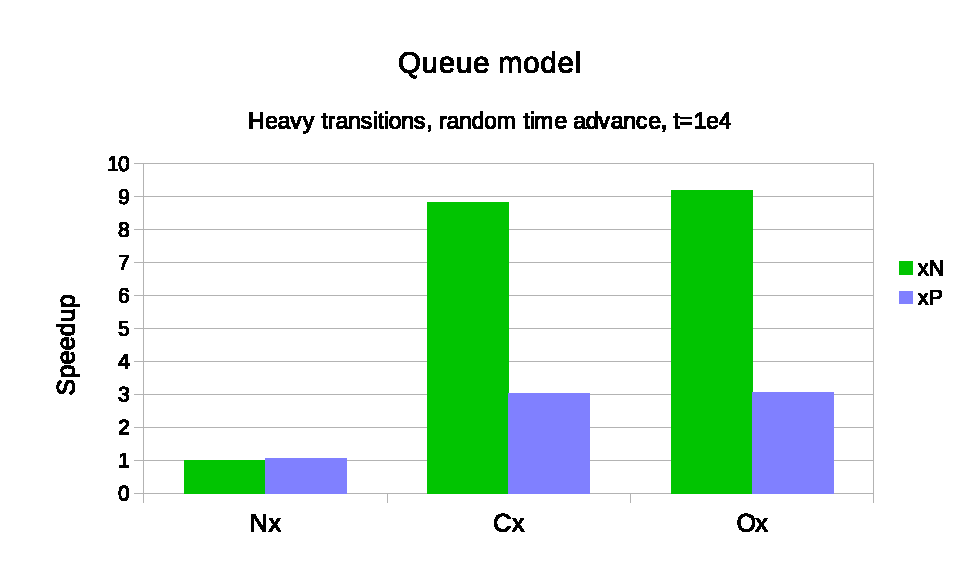
\includegraphics[width=\columnwidth]{fig/pdevs_random_sleep.eps}
	\caption{Queue speedup benchmark for PDEVS and synchronization with randomized events and significant computational load}
	\label{fig:pdevs_plot_random_sleep}
\end{figure}

\begin{figure}
	\center
	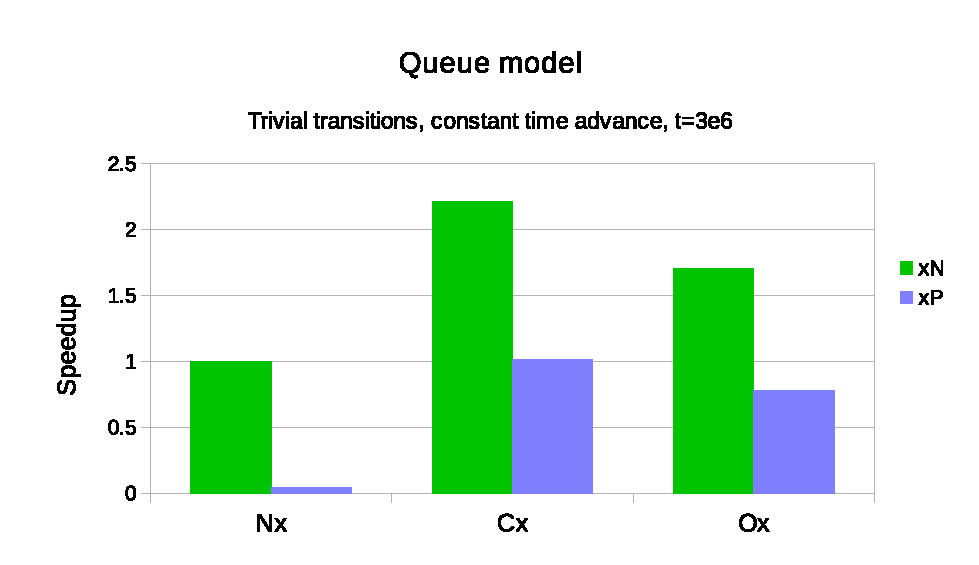
\includegraphics[width=\columnwidth]{fig/pdevs_no_sleep.eps}
	\caption{Queue speedup benchmark for PDEVS and synchronization with maximal concurrent events and trivial computational load}
	\label{fig:pdevs_plot_no_sleep}
\end{figure} 

\subsection{Memory Usage}
Apart from simulation execution time, memory usage during simulation is also of great importance.
While execution time only becomes a problem if it takes way too long, coming short only a bit of memory can make simulation unfeasible.
We therefore also investigate memory usage of different synchronization protocols, and again compare to adevs.

We do not tackle the problem of states that become too large for a single machine to hold.
This problem can be mitigated by distribution over multiple machines, which neither dxex or adevs support.

\subsubsection{Remarks}
Both dxex and adevs use \texttt{tcmalloc} as memory allocator, allowing for thread-local allocation.
Additionally, dxex uses memory pools to further reduce the frequency of expensive system calls (\textit{e.g.}, malloc and free).
\texttt{tcmalloc} only gradually releases memory back to the OS, whereas our pools will not do so at all.
Due to our motivation for memory usage analysis, we will only measure peak allocation in maximum resident set size as reported by the OS.

\subsubsection{Results}
Figure~\ref{fig:memory} shows the memory used by the different benchmarks.
Results are in megabytes, and show the total memory footprint of the running application (\textit{i.e.}, text, stack, and heap).
Note the logarithmic scale due to the high memory consumption of optimistic synchronization.

Unsurprisingly, optimistic synchronization results show very high memory usage due to the saved states.
Note the logarithmic scale that was used for this reason.
Optimistic synchronization results vary heavily depending on thread scheduling by the operating system, as this influences the drift between nodes.
Comparing similar approaches, we notice that dxex and adevs have very similar memory use.

Conservative simulation always uses more memory than sequential simulation, as is to be expected.
Additional memory is required for the multiple threads, but also to store all events that are processed simultaneously.

\begin{figure}
    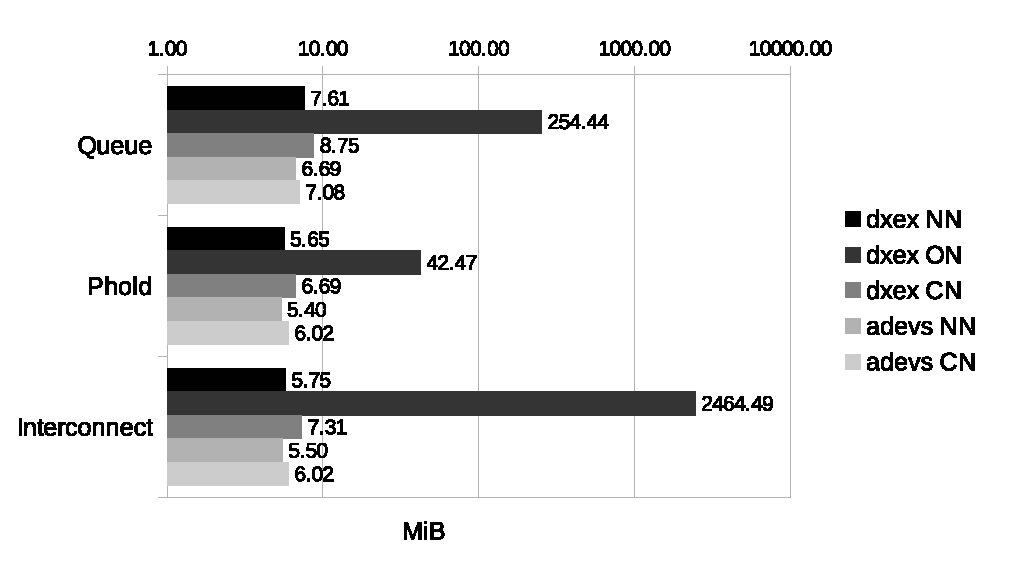
\includegraphics[width=\columnwidth]{fig/memory_voorlopig.eps}
    \caption{Memory usage results.}
    \label{fig:memory}
\end{figure}


% CONCLUSION
\subsection{Conclusion}
We have shown that our contribution is invaluable for high performance simulation: depending on the expected behaviour, modellers can choose the most appropriate synchronization protocol.
We will summarize the key aspects in achieving good parallel performance here. % reword aspects syn
\subsubsection{Allocation}
Allocation of atomic models over kernels is critical to obtain a speedup. 
In the case of the Interconnect model it is not possible to allocate models without introducing a cyclic dependency between kernels with severe performance degradation as a result. 
Even when no cycles exist in the topology between kernels a good allocation scheme will minimize the number of connections between kernels and aim for a star topology as in PHoldTree with depth first allocation or a chain topology as in the Queue model. 
Dxex can optionally offer the user a visualization of the behaviour of the kernels under a user supplied allocation scheme to allow for more insight. 
The same instrumentation could in future be used to optimize an existing allocation scheme.
\subsubsection{Uncertainty}
A simulation where future behaviour cannot be predicted is typically not suited for conservative simulation, but we have demonstrated that dxex's conservative kernel can still offer a non trivial speedup in this context. 
Optimistic is not constrained by this uncertainty and can offer a good speedup regardless of lookahead. 
Phold and PholdTree demonstrate that a single model can benefit from different synchronization protocols depending on a single parameter.
\subsubsection{Limits}
Dxex's conservative kernel is constrained by the amount of models it controls, as shown in the PHoldTree benchmark. This is especially the case when the minimal lookahead is $\epsilon$ requiring near constant polling of models for lookahead values. 
Optimistic is not constrained by the number of models it manages, but can quickly consume all available memory in a simulation. While this effect can be reduced with a thread aware allocation scheme, the underlying problem remains.




\section{Model Allocation}
\label{sec:4a-allocation}
Although the synchronization protocol is one of the defining factors in simulation performance, model allocation has a significant impact on which protocol is ideal, and even whether or not parallelization would make sense.
Indeed, if the model is distributed in such a way that frequent communication is necessary between cores, parallelism is naturally reduced.
This thus brings us to the topic of model allocation.
Model allocation was one of the features also implemented by PythonPDEVS~\cite{PythonPDEVS2}.

The modeller can specify which kernel a model should be allocated to, should such manual intervention be required.
This is handled by the default model allocator.
If no preference is given a simple striping scheme is followed but this is not sufficient in most simulations to achieve a speedup in parallel.
By overriding the default allocator a modeller tunes the allocation scheme for a specific model, maximizing parallel speedup.
This interface can be used to employ graph algorithms for an automatic allocation scheme, for example avoiding cycles in the dependency graph.

\subsection{Performance Evaluation}
%TODO do basic performance evaluation of allocation
%TODO show model in statistics view
In order to evaluate the influence of model allocation, we define a new model, based on PHOLD~\cite{PHOLD}.
The model structure resembles a tree: an atomic model can have a set of children, with children being connected to each other as well.
Connections can be uni- or bidirectional.

Unlike the Queue model, the width of the hierarchy is still present in the topology of the atomic models after the direct connection stage.
The PHOLDTree model allows us to investigate parallel speedup in terms of model allocation, by modifying the depth and width (fanout) model parameters.

The PHOLDTree model is similar in structure to models of gossiping in social networks~\cite{?}, hierarchical resource sharing~\cite{?} or load balancing~\cite{?}.
The lookahead of an atomic node is the minimally allowed $\epsilon$, indicating uncertainty, as is often the case in realistic models.
We demonstrate the importance of allocation, by comparing a breadth-first versus a depth-first scheme.

\begin{figure}
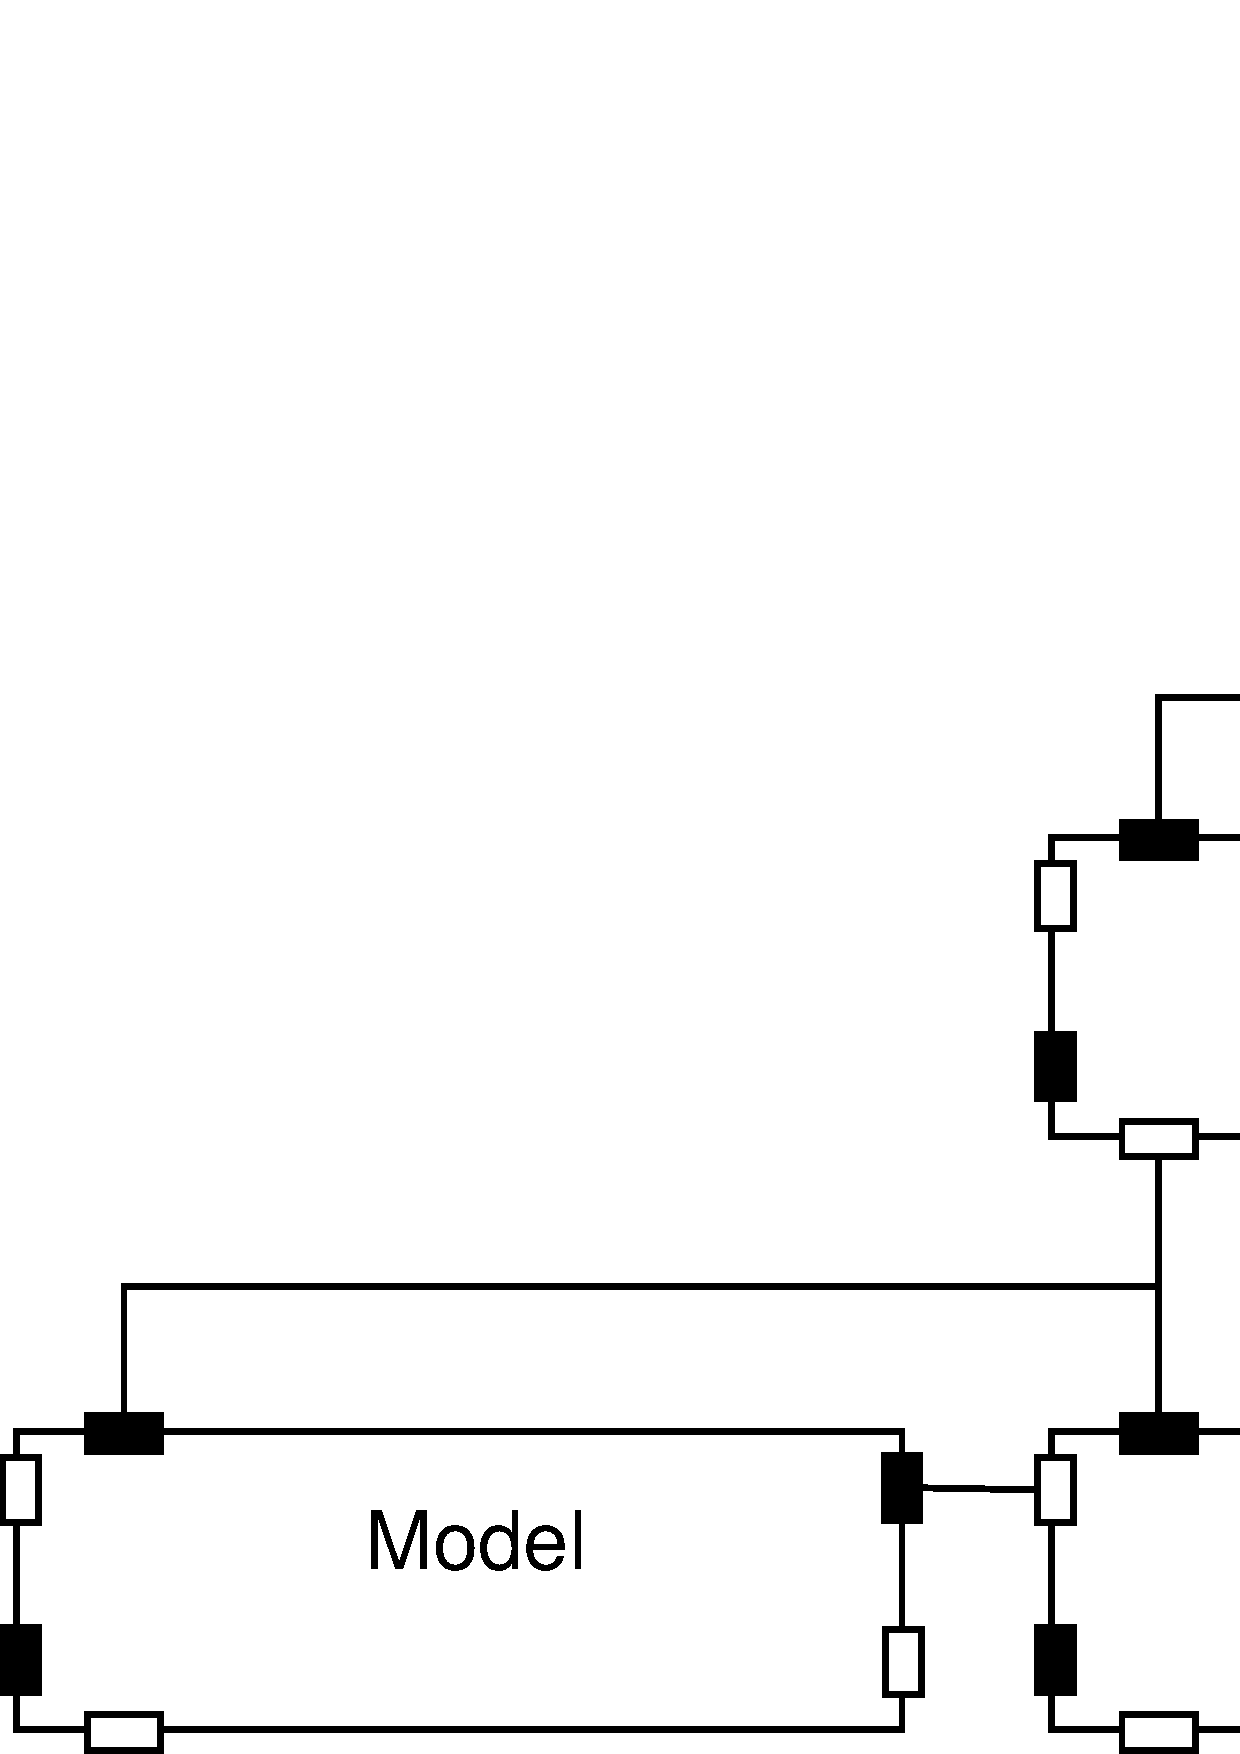
\includegraphics[width=\modelfraction\columnwidth]{fig/pholdtree.pdf}
%TODO depth 1 but 3 levels deep?
\caption{PHOLDTree model for depth 1 and width 2.}
\label{fig:PHOLDTree_model}
\end{figure}

PHoldtree, like Queue, is a highly hierarchical model but one where the flattened structure cannot be partitioned into a chain as in Queue.
This topology is interesting since it highlights the effects of allocation.
This model allows us to investigate in depth the effects of non-cyclic allocation strategies and measure parallel speedup.
First, we evaluate the model in sequential simulation to provide a baseline for parallel simulation.

\subsubsection{Sequential Simulation}
Since adevs does not use direct connection, we expect a noticable performance difference between dxex and adevs.
This is shown in Figure~\ref{fig:PHOLDtree_seq_dn_benchmark}, where the fanout determines the performance penalty adevs suffers compared to dxex.
Profiling indeed indicated that an increase in width per subtree ($n$) leads to higher overheads in adevs due to the lack of direct connection.
Dxex uses direct connection, making it independent on fanout, but only of the number of models.
Slight deviations can still be seen, though, caused by the initialization overhead of direct connection.
Both adevs and dxex scale linearly in the number of atomic models.
We expect to see a similar distinction in parallel simulation.

\begin{figure}
    \center
    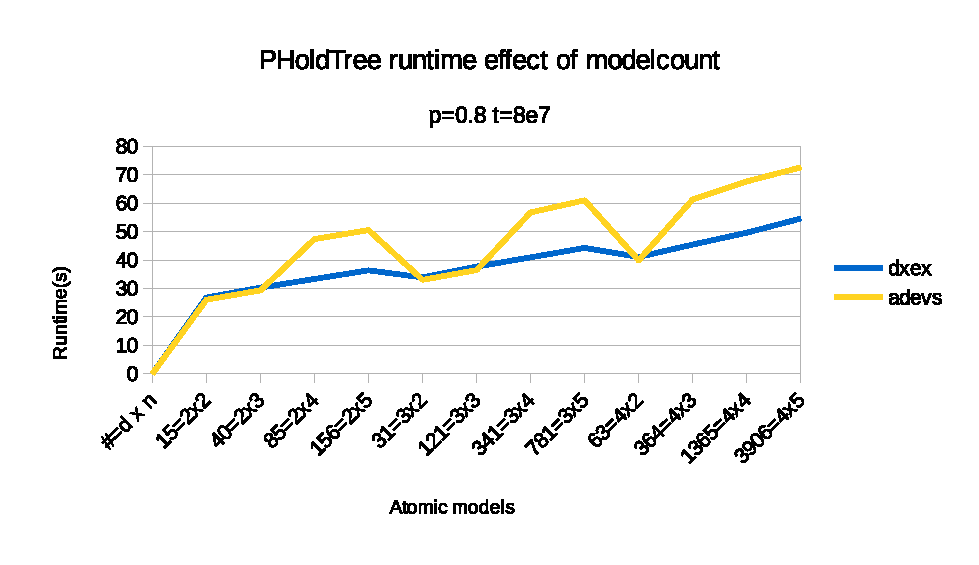
\includegraphics[width=\plotfraction\columnwidth]{fig/pholdtree_sequential_dn.eps}
    \caption{Effect of hierarchy in sequential simulation.}
    \label{fig:PHoldtree_seq_dn_benchmark}
\end{figure}

\subsubsection{Parallel Simulation}
Next, we run the model using two different model allocation schemes: breadth-first and depth-first.
But first, we explain what we mean by both allocation schemes.

With breadth-first allocation, we traverse the tree in a breadth-first way, allocating subsequently visited atomic models to the same node.
This means, intuitively, that atomic models at the same level in the tree, but not necessarily siblings, are frequently allocated to the same node.
Since there is only infrequently some communication between 
This allocation strategy is shown in Figure~\ref{fig:BF}.

With depth-first allocation, we traverse the tree in a depth-first way, allocating subsequently visited atomic models to the same node.
This means, intuitively, that subtreees are frequently allocated to the same node.
This allocation strategy is shown in Figure~\ref{fig:DF}.

The breadth first allocation scheme will result in kernels that will form a dependency chain with multiple branches, much like in the Queue model.
Such a linear dependency chain can result in a parallel speedup as we demonstrated with the Queue model, but this is not always true as we will demonstrate in this section.
A single kernel that has an unbalanced number of atomic models or unequal computation load in transition functions will slow down the remainder of the chain. This effect is also apparent if the thread a kernel runs on is not fairly scheduled. In conservative this will lead to excessive polling of the other kernels' eot values, in optimistic this will lead to a cascade of reverts since dependent kernels will simulate ahead of the slower kernel. In Figures \ref{fig:pholdtree_visualize_parBFS} and \ref{fig:pholdtree_visualize_parDFS} the simulation trace is visualized for both allocation schemes highlighting the remarks made in this paragraph.
\begin{figure}
   \center
   
   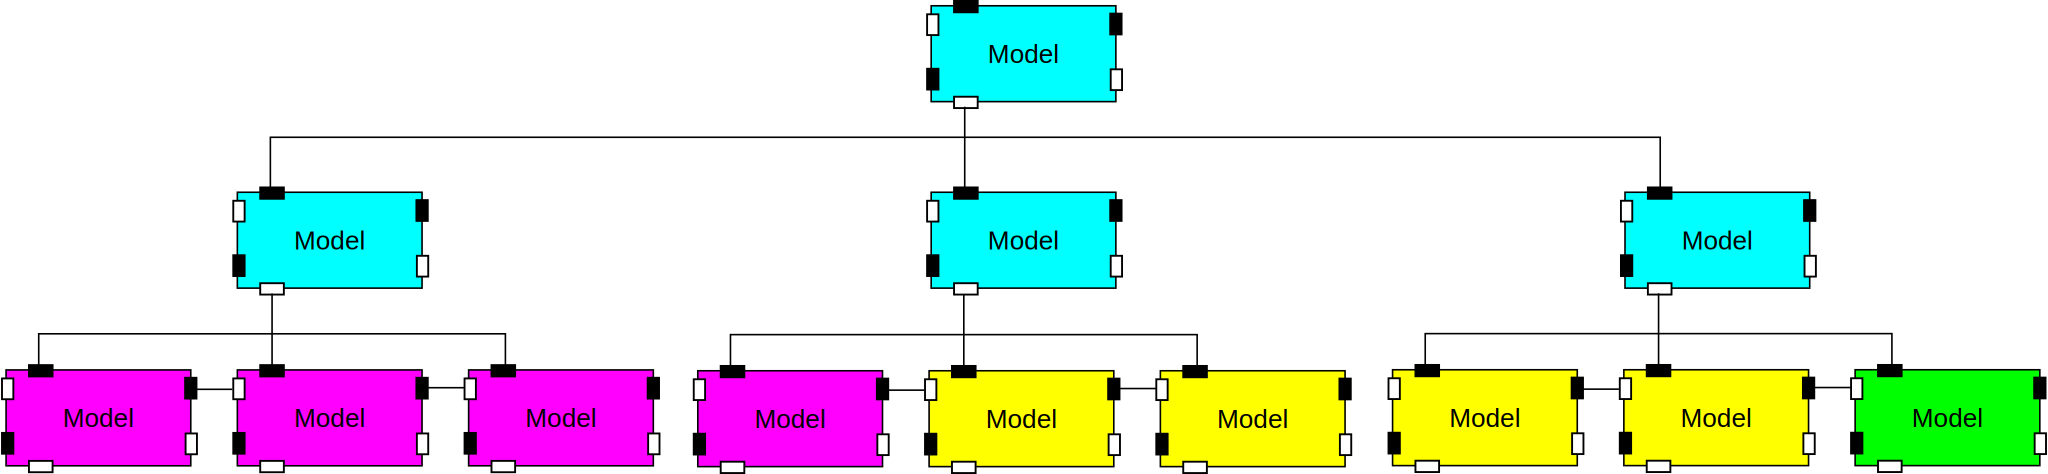
\includegraphics[width=\modelfraction\columnwidth]{fig/pholdtree_alloc_BF.pdf}
   \caption{PholdTree model breadth first allocation with 4 kernels.}
   \label{fig:PholdTree_model_bfs}
   \includegraphics[width=\modelfraction\columnwidth]{fig/pholdtree_alloc_DF.pdf}
   \caption{PholdTree model depth first allocation with 4 kernels.}
   \label{fig:PholdTree_model_dfs}
\end{figure}

After simulation, the traces can be visualized for both breadth-first and depth-first allocation.
Using a breadth-first allocation scheme, as shown in Figure~\ref{fig:pholdtree_visualize_parBFS}, we notice that many events get exchanged between cores.
This is caused by the high number of inter-core connections and the high number of events exchanged over these connections.
The number of connections between nodes at the same simulation core is also rather low.
Using a depth-first allocation scheme, however, as shown in Figure~\ref{fig:pholdtree_visualize_parDFS},

\begin{figure}
    \center
    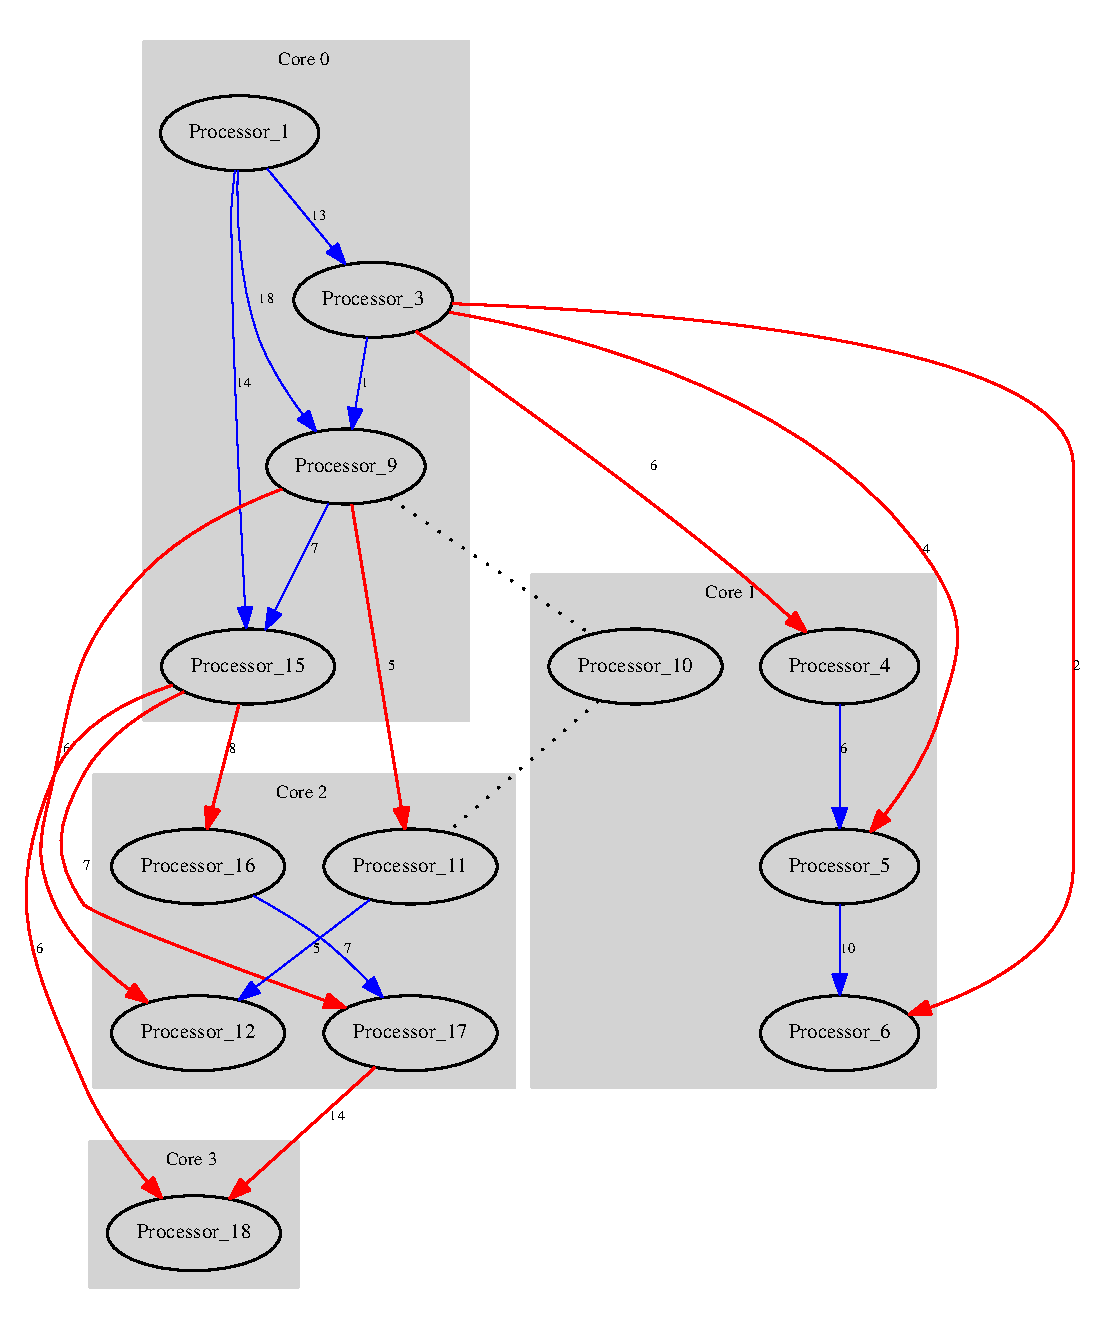
\includegraphics[width=\plotfraction\columnwidth,  height=6cm, keepaspectratio]{fig/pholdtreed1n3t5000c4BFS.eps}
    \caption{Visualization of PholdTree (d=1,n=3,t=5000) parallel simulation with breadth first allocation and 4 kernels.}
    \label{fig:pholdtree_visualize_parBFS}
\end{figure}
\begin{figure}
    \center
    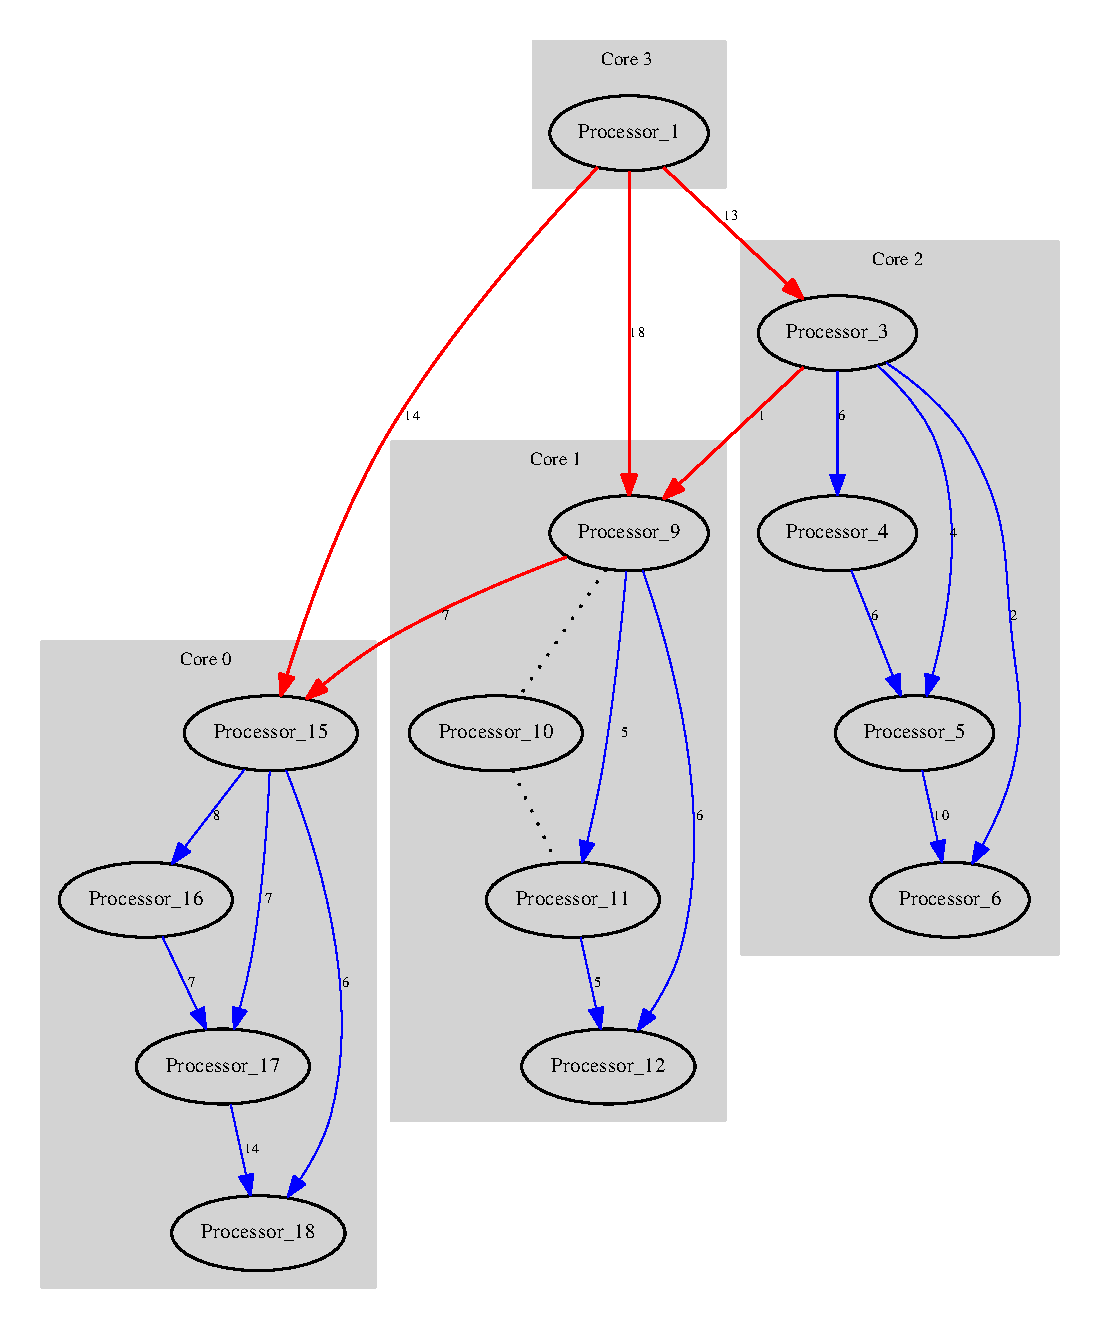
\includegraphics[width=\plotfraction\columnwidth,  height=6cm, keepaspectratio]{fig/pholdtreed1n3t5000c4DFS.eps}
    \caption{Visualization of PholdTree (d=1,n=3,t=5000) parallel simulation with depth first allocation and 4 kernels.}
    \label{fig:pholdtree_visualize_parDFS}
\end{figure}

Simulation results are shown in Figure~\ref{fig:?} for both allocation schemes in combination with both synchronization protocols.
We see that for both synchronization protocols, the depth-first allocation is significantly better than breadth-first allocation.
This is what we expected: depth-first allocation maintains locality better than breadth-first allocation.

%TODO this paragraph is strange: is this really the case?
Interestingly, we see that optimistic synchronization is less influenced by the allocation than conservative synchronization.
This is likely caused due to the lower number of connections to take into account in conservative synchronization.
Whereas conservative synchronization needs to take into account even scarcely used connections, optimistic synchronization does not.
The same is true in the opposite direction, though, where optimistic synchronization is slower when a good allocation is chosen.
Conservative synchronization will then be able to make better estimates, whereas optimistic synchronization does not make estimations.

\paragraph*{Strong Scaling}\label{pholdtreestrongscale}
In Figure \ref{fig:PholdTree_plot_alloc_high} we see that the difference in performance for all 4 kernel configurations compared to that shown in Figure \ref{fig:PholdTree_plot_alloc_low} is a constant factor. The probability of the priority message has no extra impact on performance other than that shown in sequential performance.

The probability of a high priority event in this model does not affect the performance difference between conservative and optimistic. The key parameter quickly becomes the load of a kernel in models. Our conservative implementation in an uncertain simulation is very sensitive to a high load in models, whereas optimistic has no such limitation.

The difference between depth first and breadth first allocated kernels is striking, the first results in sublinear speedup for both synchronization protocols. %reword 
The breadth first allocation scheme will lead to a very high number of inter-kernel connections, which is detrimental for any parallel synchronization algorithm. An event exchanged between kernels cannot be securely deallocated without a GVT algorithm and all the complexity this entails. Even a fast asynchronous GVT algorithm will require some form of inter kernel synchronization and span a timeframe during which allocated memory cannot be reused, forcing new allocations.
Similar to the Queue benchmark the breadth first allocation scheme leads to a topology for the kernels resembling a chain but with more branches in the chain. In Queue there is only a single model on the edge of a kernel exchanging messages to a single other model in a neighbouring kernel, this is not the case in the PholdTree under breadth first allocation. This explains the difference in speedup between Queue and PholdTree despite the similarity in kernel topology.\\
Depth first allocation still has a higher inter kernel connection count, but not on the same order as breadth first allocated PholdTree. Depth first allocation will converge to a star topology which in this benchmark leads to a significant speedup.\\
The performance drop observed for 2 kernels for all allocation schemes and synchronization protocols is in part due to the higher link count between kernels. With more kernels these connections will be spread across more kernels and result in a relative lower performance penalty. \\
Conservative synchronization suffers a further penalty in this benchmark when there are only a few kernels. The PholdTree model has a lookahead of $\epsilon$ leading the kernel to query each allocated atomic model for a lookahead value on each simulation round. As the atomic models are spread over more kernels this effect is reduced leading to an increase in performance. With 4 kernels conservative surpasses optimistic in speedup. This is clear evidence that conservative synchronization is a good candidate for parallel simulation even in simulations with uncertainty.
\begin{figure}
    \center

    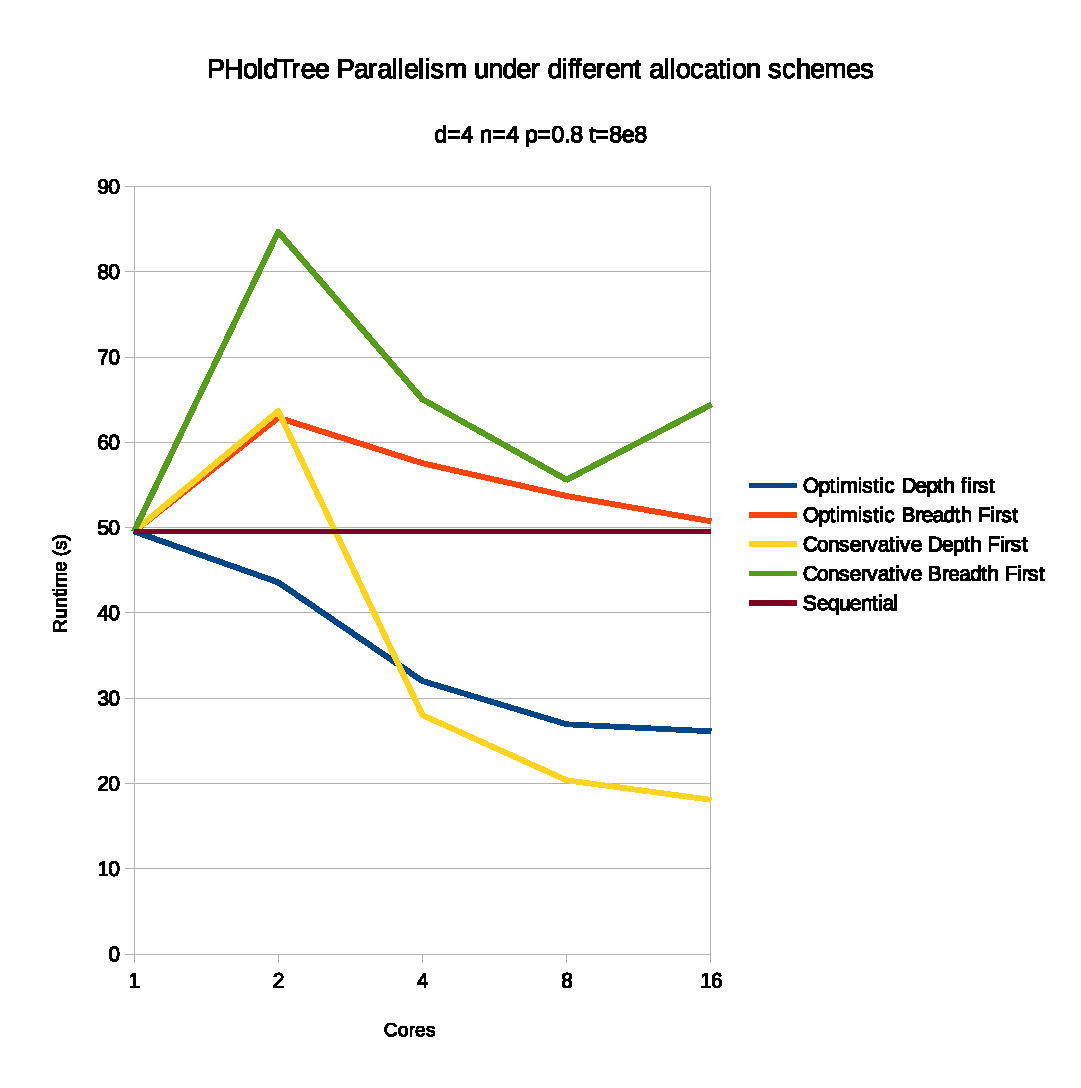
\includegraphics[width=\modelfraction\columnwidth]{fig/pholdtreealloclowp.eps}
    \caption{PholdTree model performance under different allocation schemes with low message probability}
    \label{fig:PholdTree_plot_alloc_low}

    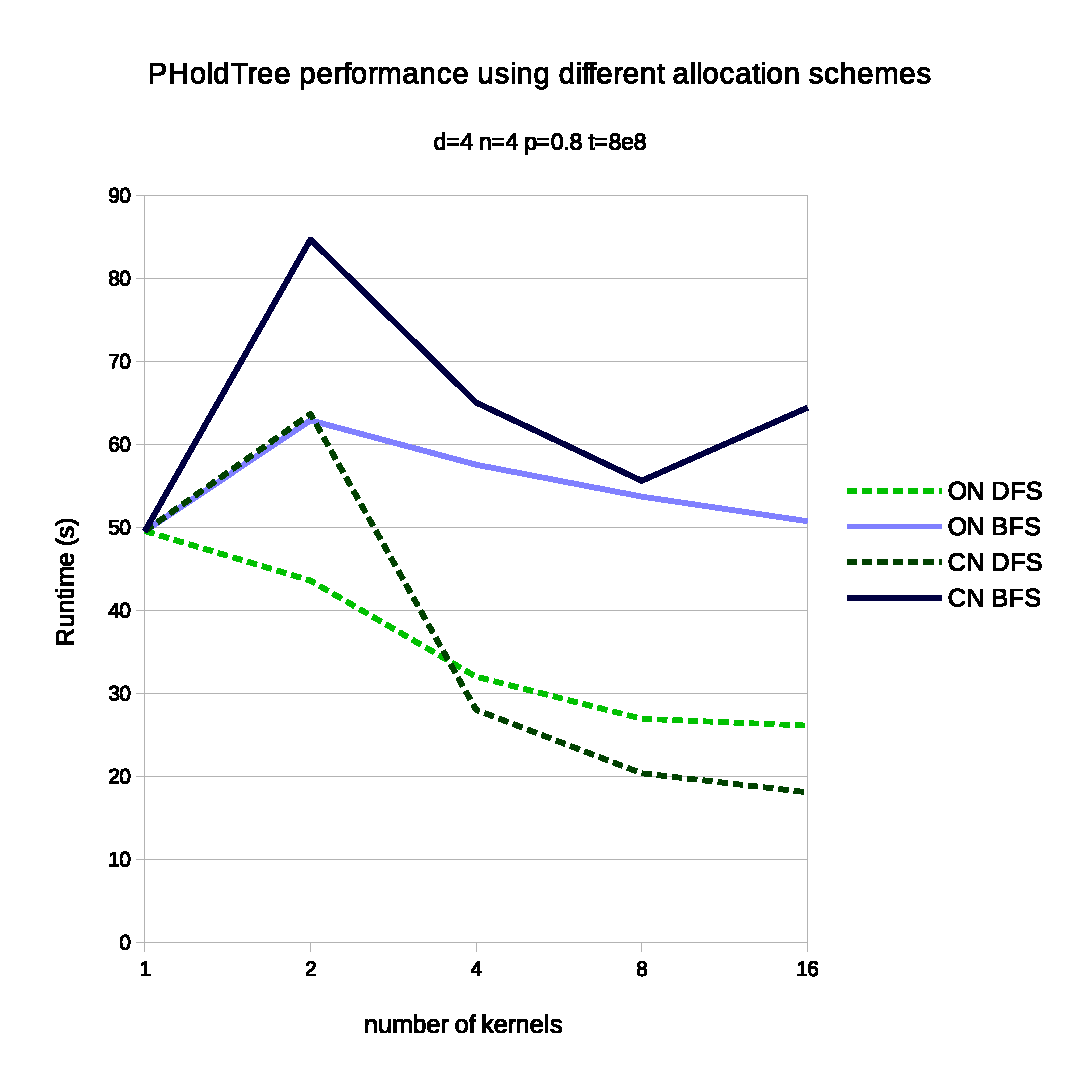
\includegraphics[width=\modelfraction\columnwidth]{fig/pholdtreeallochighp.eps}
    \caption{PholdTree model performance under different allocation schemes with high message probability}
    \label{fig:PholdTree_plot_alloc_high}
\end{figure}

\paragraph*{Weak Scaling}
%Intro
In this paragraph we investigate dxex's parallel performance when the the number of atomic models distributed over a fixed number of kernels varies. From \ref{eq:pholdtreemodelcount} we know that increasing d will lead to a very rapid increase in models. We want to observe what happens in a closer to linear increase in model count per kernel by varying n.

% Explain why adevs is not plotted (its x100 slower)
Adevs' conservative implementation cannot handle the uncertainty (lack of non $\epsilon$ lookahead) here and is omitted from the comparison. Its parallel performance is two orders of magnitude slower than the sequential implementation. Upon investigation we conclude that this slowdown is caused by not implementing the \{begin/end\}lookahead() functions, which when not overridden in a model trigger an exception on each invocation.
This exception handling completely stalls the kernel. We do not implement this function in our PholdTree variant for adevs since this would force us to implement state saving in the model code and not use the provided state saving functionality in the kernel, as is done in dxex or PythonPDEVS's optimistic.
In dxex state saving is never required for a conservative simulation, this is handled transparently for the user who need not implement this behaviour.
By using the state saving technique inside the model code we feel we would no longer compare identical models across different synchronization algorithms, although we do not doubt adevs' increased performance when these functions are overridden.

% Optimistic
In Figure \ref{fig:PholdTree_plot_weaknopt} we observe that dxex's optimistic kernels are slightly sensitive to the number of atomic models allocated to them. In the worst case with 2 kernels there is no real speedup observable, as soon as the number of kernels increases we see a converging speedup trend, that except for 32 kernels is almost constant despite the increase in n. Note that only depth first allocated kernels are measured here, breadth first as we can see in \ref{fig:PholdTree_plot_alloc_high} has no speedup advantage. The probability parameter is kept at 0.1 for the same reason, it only induces a linear increase in load.

% Conservative
Conservative has a more nuanced speedup behaviour in this benchmark. We have detailed how a conservative kernel in dxex scales linear in the number of atomic models (if lookahead is $\epsilon$), this effect is more clearly visible here. \\
It is clear that as the fanout (n) of the model increases the kernel performance degrades rapidly. The intersection of the performance graph of each configuration is shifted to the right, the actual 1-speedup point increases as the kernelcount increases. For a d=4, n=5 configuration with 4 kernels each kernel has a load of ~1300 atomic models when it crosses the 1-speedup line. \\
An 8 kernel configuration with d=4 n=6 can sustain a load of ~2700 atomic models before it reaches that point. From the results we see that the 32-kernel configuration is not yet slowing down with the current parameters. \\
The modelcount is only a part of the explanation of this effect, as the kernelcount increases the amount of inter kernel messages will be split into more distinct sets which can be handled with more concurrency in dxex's architecture.
That this effect is not always true can be observed from the d=4 n=3 32-kernel datapoint. Note that in this configuration 341 atomic models are distributed over 32 kernels, a relative low model load can more easily highlight synchronization overhead, even if allocation is optimal.\\
As with optimistic we do not include breadth first allocated benchmarks in this speedup plot since none of those achieve a speedup higher than 1.
\\
If we combine both to determine which synchronization protocol is more optimal we see in Figure \ref{fig:PholdTree_plot_weakall} that for these configurations conservative with 8 kernels is an ideal configuration up until n=5, where the modelcount starts to degrade performance. Optimistic with the same kernelcount is almost insensitive to the increase in modelcount and is therefore a more robust choice. Note how optimistic and conservative with 32 kernels at this point still have a reasonable speedup which is surprising given the synchronization overhead in such a large set of kernels.
\begin{figure}
    \center

    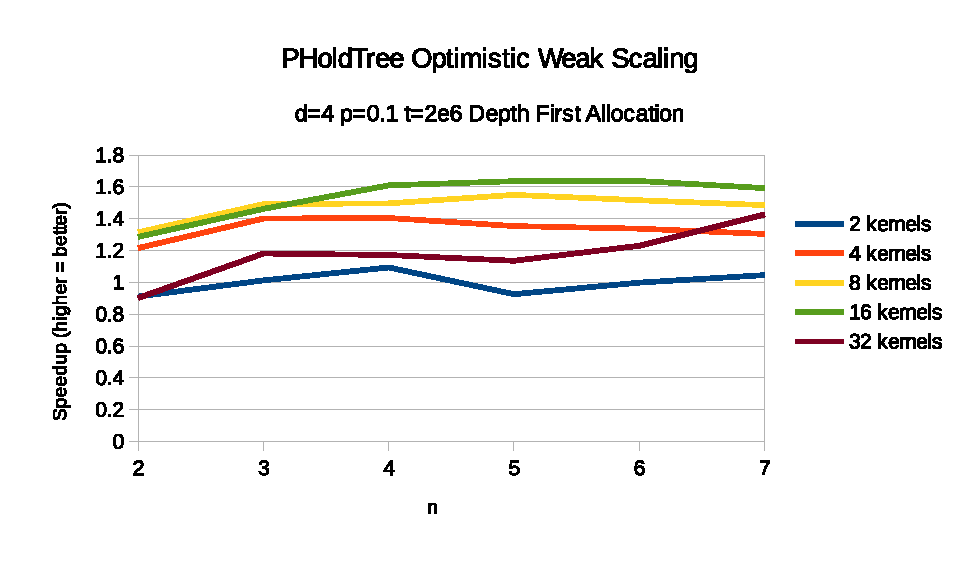
\includegraphics[width=\modelfraction\columnwidth]{fig/pholdtreeweakscalingnopt.eps}
    \caption{PholdTree model weak scaling under varying fanout and optimistic synchronization}
    \label{fig:PholdTree_plot_weaknopt}

    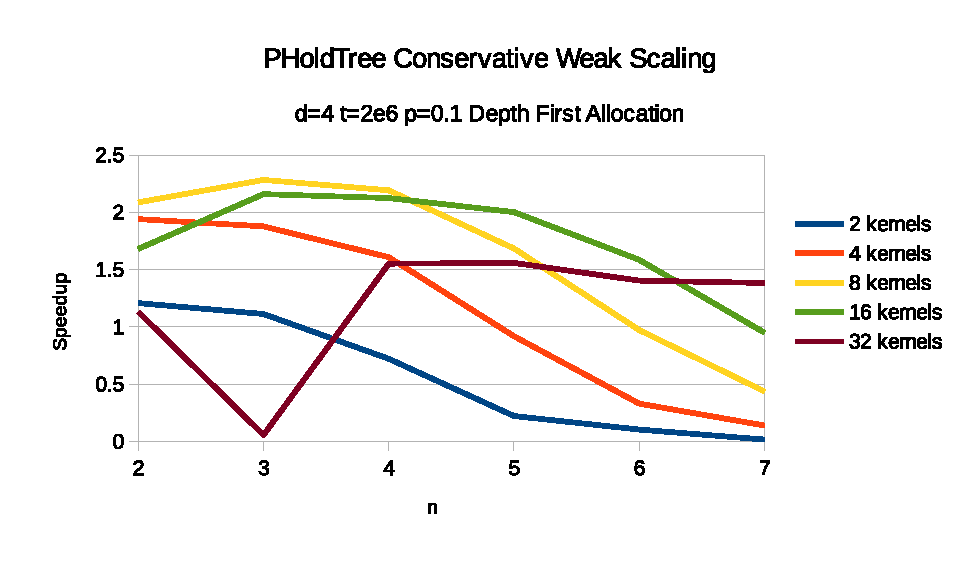
\includegraphics[width=\modelfraction\columnwidth]{fig/pholdtreeweakscalingncon.eps}
    \caption{PholdTree model weak scaling under varying fanout and conservative synchronization}
    \label{fig:PholdTree_plot_weakncon}

    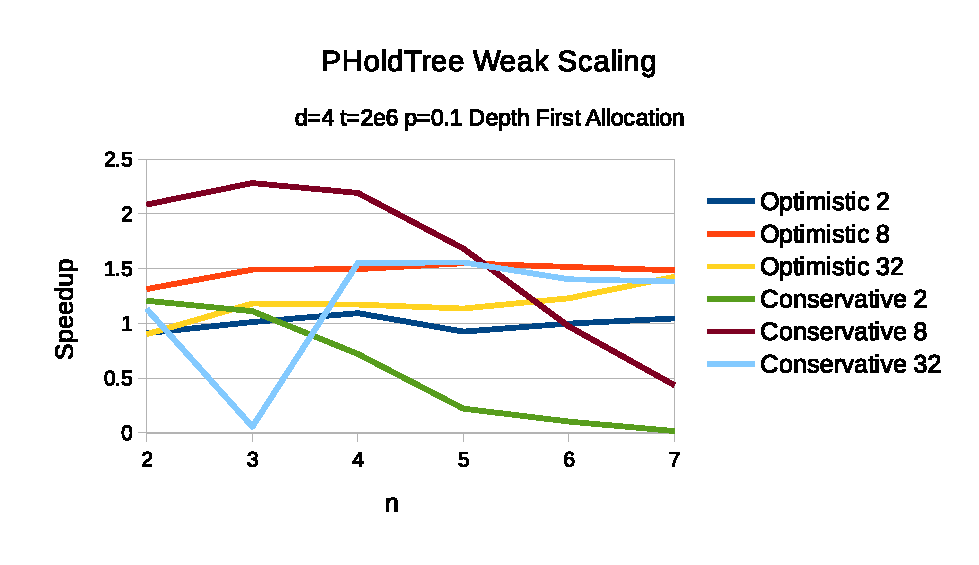
\includegraphics[width=\modelfraction\columnwidth]{fig/pholdtreeweakscalingall.eps}
    \caption{PholdTree model weak scaling under varying fanout and different synchronization algorithms}
    \label{fig:PholdTree_plot_weakall}
\end{figure}

\subsection{Linking Back}
%TODO link back to initial performance evaluation



\section{Hotswapping the Synchronization Protocol}
\label{sec:4b-hotswap}
%TODO explain hotswapping
%TODO why hotswapping
Simply because a synchronization protocol is ideal at the start of the simulation, does not mean that it will still be ideal during the simulation.
It has been frequently shown, and repeated in the previous section, that model behaviour significantly influences the ideal synchronization protocol.
Contrary to many modelling formalisms, the DEVS formalisms makes it possible to model basically any kind of discrete event model.
As such, it is possible for the model to significantly change its behaviour throughout the simulation.

Defining the ideal synchronization protocol at the start of the simulation, when information about future model behaviour might be scarce, might therefore not offer the best possible performance.
In dxex, we not only make it possible to define the synchronization protocol to use, but also to change this decision throughout simulation.
To do this, all kernels are notified of the switch and they are forced to stop simulation using the current synchronization core.
When stopped, each kernel instantiates a new core that is provided with the simulation state of the previous core.
Simulation is then resumed with the new cores after the previous ones are destroyed.

As usual, switching imposes an overhead and should thus only be done if the benefits outweigh the induced overhead.
This overhead depends on the size of the model and the number of simulation cores.
For a simple model and a few cores, the overhead is less than a single second.

Although we currently only support manual switches between different synchronization protocols, this is not necessarily the case.
Ideally, a new component is added to the simulation kernel, which monitors model behaviour and simulation performance, and toggles between them automatically.
Our interface is thus augmented with the necessary bindings for such a component to be defined.
Also, our interface is augmented with an interface for statistics gathering and model behaviour analysis.
The implementation of such a component is currently left open: algorithms can be heavily based on machine learning or similar approaches.

\subsection{Statistics Gathering}
Traditionally, models are not exposed to simulation kernel details due to the wrong level of abstraction.
Simulation models only care about being simulated, and not about how this is being done.
This is different for a new simulation kernel component that has to monitor the behaviour of not only the model, but the simulator as well.

We add performance metrics in the simulation kernel, which logs relevant performance metrics and processes them for use in other components.
These metrics include the number of events created and destroyed, the number of inter and intra kernel events, the number of rollbacks, the measured lookahead, details of the Global Virtual Time (GVT) and Earliest Output Time (EOT) calculations, and basic information on the fairness between different simulation kernels.
With all these metrics, a component can get a fair view on both model and simulation kernel behaviour.

For example, if the actually seen lookahead is significantly higher than the defined lookahead, it might be interesting to switch to optimistic synchronization.
When the number of rollbacks is very high, conservative synchronization might be ideal.
And when neither of these two is an option, the simulation might just (temporarily) have to fall back to sequential simulation.

For performance reasons, statistics gathering is optional due to the imposed overhead.

\subsubsection{Visualization of Communication}
To provide some more insight in the models we used as benchmarks previously, we created a simple visualization of the simulation trace.
This trace visualizes the allocation of the model and all defined connections.
For each connection, the number of events transferred is annotated.
Examples are shown for the three benchmark models used before: Figures~\ref{fig:Queue_allocation},~\ref{fig:interconnect_allocation_parallel}, and~\ref{fig:phold_allocation} shows traces for the Queue, Interconnect, and PHOLD models respectively.

\begin{figure}
    \center
    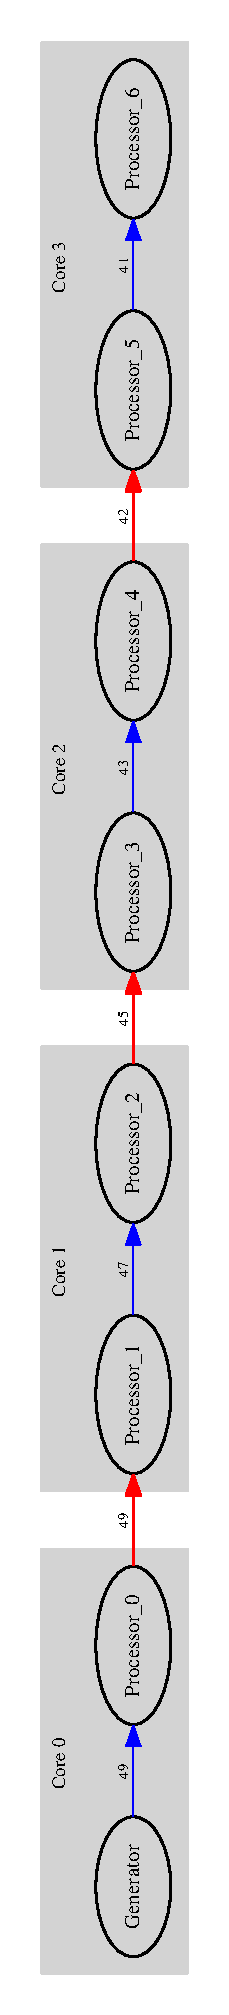
\includegraphics[width=\modelfraction\columnwidth, height=8cm, keepaspectratio, angle=-90 ]{fig/queue_allocation.eps}
    \caption{Queue model (d=2, w=7, t=5000, random timeadvance) allocation and simulation trace across 4 kernels.}
    \label{fig:Queue_allocation}
\end{figure}
\begin{figure}
    \center
    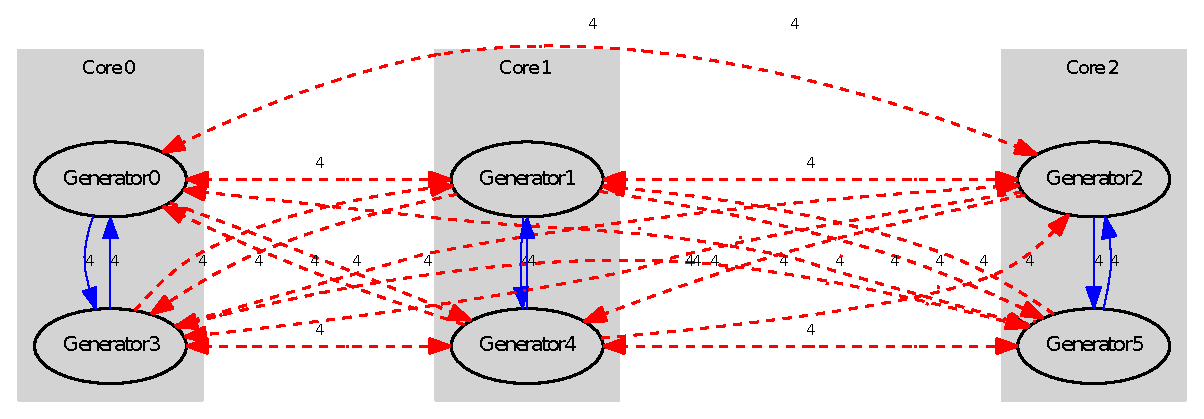
\includegraphics[width=\plotfraction\columnwidth]{fig/interconnect_parallel_allocation.eps}
    \caption{Interconnect parallel simulation trace for 6 models on 3 kernels.}
    \label{fig:interconnect_allocation_parallel}
\end{figure}
\begin{figure}
    \center
    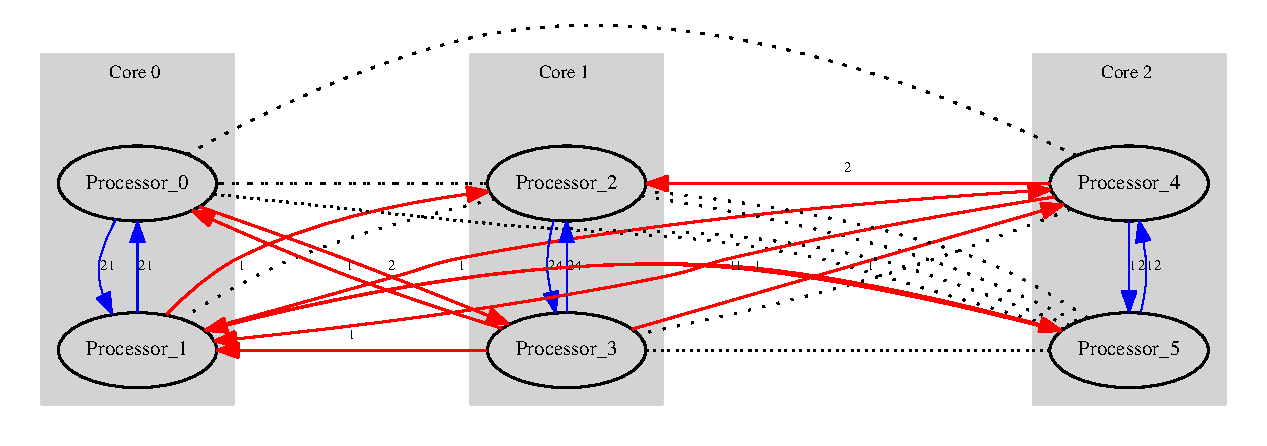
\includegraphics[width=\plotfraction\columnwidth]{fig/phold_parallel_allocation.eps}
    \caption{Phold benchmark trace for parallel simulation using three kernels.}
    \label{fig:phold_allocation}
\end{figure}

Naturally, results similar to this are relevant information that can be used by the hotswapping component.


\section{Related Work}
\label{sec:5-related-work}
%TODO explain about other DEVS simulation kernels, and how they differ
%TODO explain about PythonPDEVS, the most related in terms of feature and "legacy" --> now in C++11 and way better performance
\subsection{PythonPDEVS}
Dxexmachina is closely related to PythonPDEVS in design and philosophy. PythonPDEVS allows anyone who grasps the DEVS formalisms to immediately simulate his/her model without having to consider the kernel implementation. C++ implementations cannot hope to match the fast prototype/edit/run cycles provided by PythonPDEVS, although this can be minimized by building the kernels as libraries. %maybe warn that if a header is touched, you still have to compile from scratch ? (eg. TIME_FP)
Advanced features such as activity based relocation and the performance gains this results in, are still unique to PythonPDEVS.
\subsection{Adevs}
%TODO explain about adevs, the most related in terms of performance --> we implement more synchronization options and offer better performance because ...
Adevs's source code is still under active development, allowing for an exact comparison in performance and features. It remains in most aspects the fastest simulation engine for the DEVS formalism, but it lacks an optimistic synchronization implementation. %Tracing ?
By virtue of not flattening Coupled Models, performance suffers in increasingly hierarchical models.
%checkme
\subsection{CD++}
%TODO explain about CD++, the most related in terms of synchronization --> we implement everything in a single program, with a non-fragmented code-base
%TODO make mention of Warped, which is the kernel used in CD++, and why we don't use it
Different projects on CD++ offer conservative (CCD++) as well as optimistic (PCD++) parallel simulation. In contrast to our single program, with a non-fragmented code-base, neither projects offer both synchronization protocols. CD++ relies on the WARPED kernel. It is a middleware that provides memory, event, file, time and communication scheduling. WARPED is not used here since we operate explicitly on a shared memory system and since we wanted to design our kernels using the least amount of overhead possible.


\section{Conclusions and future work}
\label{sec:6-conclusion}
In this paper, we introduced dxex, a new C++11-based \textsf{Parallel DEVS} simulation tool.
Our main contribution is the implementation of different pluggable synchronization kernels for parallel simulation.
We have shown that there are indeed models which can be simulated significantly faster using either synchronization protocol.
Dxex allows the user to chose between both conservative and optimistic synchronization, as simply as any other configuration option.
Notwithstanding this modularity, we have shown that dxex achieves performance similar to adevs, another very efficient \textsf{DEVS} simultion tool.
Performance is measured both in CPU time, and memory usage.

Future work exists in several directions.
First, we wish to make optimistic synchronization more tolerant to low-memory situations.
In its current state, simulation will simply halt with an out-of-memory error.
Having simulation control, which can throttle the speed of nodes that use up too much memory, has been shown to work in these situations~\cite{FujimotoBook}.
In our implementation specifically, the out-of-memory problem is aggravated by a slow GVT implementation.
Algorithms as those presented by~\cite{Fujimoto:1997:CGV:268403.268404} or~\cite{Bauer:2005:SND:1069810.1070159} might help to alleviate this problem.
Second, the idea of activity can be implemented for our simulation kernels, making it possible to dynamically switch between conservative and optimistic synchronization when changes in the model behaviour are detected.
Third, activity algorithms, as already implemented by PythonPDEVS, could also be implemented in dxex, to determine how they influence simulation performance.


\section*{ACKNOWLEDGMENTS}
This work was partly funded with a PhD fellowship grant from the Research Foundation - Flanders (FWO). 

\bibliographystyle{SageV}
\bibliography{papers}

\end{document}
